\documentclass[a4paper,12pt]{article}

%PACKAGES

\usepackage[T1]{fontenc}
\usepackage{lmodern}

\usepackage[utf8]{inputenc}
\usepackage[slovak]{babel}
\usepackage{comment}

\usepackage{graphicx,amsmath,amssymb, amsthm, multicol}
\usepackage{pdfpages}

\usepackage[nottoc]{tocbibind}
\usepackage{mathrsfs}
\usepackage{psfrag}
\usepackage[small,bf]{caption}
\usepackage{ifthen}

\usepackage{xcolor}
\usepackage{listings}
\usepackage{enumitem}

\usepackage[toc,page]{appendix}

\usepackage{url}
\urlstyle{rm}
\renewcommand\UrlFont{\color{black}}

\usepackage{tikz}
\usetikzlibrary{positioning,chains,fit,shapes,calc}

% \renewcommand{\familydefault}{\rmdefault}

\newtheorem{defin}{Definícia}[section]
\newtheorem{theorem}[defin]{Veta}
\newtheorem{prop}[defin]{Tvrdenie}
\newtheorem{lema}[defin]{Lema}
\newtheorem{cor}[defin]{Dôsledok}
\newtheorem{hypoteza}{Hypotéza}[section]
\newtheoremstyle{comment}{}{}{}{}{}{:}{ }{#1}
\theoremstyle{comment}
\newtheorem{dokaz}{Dôkaz}[section]
\newtheorem{com}{\textit{Poznámka}}

\usepackage{hyperref}                                     
\hypersetup{%  http://www.tug.org/applications/hyperref/
bookmarksnumbered,
pdfstartview={FitH},
linkcolor=black,
citecolor=black,
colorlinks=true,
pdfpagemode={None},
plainpages=false
}%

%%\usepackage{fullpage}
%%\setlength{\topmargin}{-0.5cm}
%%\setlength{\headheight}{0cm}
%%\setlength{\headsep}{0in}
\setlength{\textheight}{24cm}
\setlength{\textwidth}{15.5cm}
\addtolength{\voffset}{-1.2cm}
\addtolength{\hoffset}{-0.3cm}
%%\addtolength{\rightmargin}{-1cm}
\setlength{\parindent}{0.5cm}
\setlength{\parskip}{0in}
\linespread{1.5}

\setcounter{MaxMatrixCols}{20}

\begin{document}

  \thispagestyle{empty}
\begin{center}
{\large \bf UNIVERZITA KOMENSKÉHO V BRATISLAVE \\
FAKULTA MATEMATIKY, FYZIKY A INFORMATIKY}
\end{center}
%\begin{titlepage}
%    \rmfamily
%    \begin{center}
%      \LARGE\scshape
%      \theuniversity\\
%      \Large\upshape
%      \thefaculty\\
%      \large
%      \thedepartment
%    \end{center}
%

\vspace{2cm}
\begin{figure}[!h]
   \centering
     %
\includegraphics[width=3.5cm]{logoUK.jpg}
\end{figure}

\vspace{1cm}
\begin{center}
{\large \bf Riadkovo-stĺpcové návrhy štatistických experimentov \\
\vspace{3cm}
BAKALÁRSKA PRÁCA}
\end{center}

\vfill
%
\begin{multicols}{2}
{\bf
\begin{flushleft} 2020 \end{flushleft}
\begin{flushright} Róbert Druska \end{flushright} 
}
\end{multicols}


  \newpage
\thispagestyle{empty}
\begin{center}
{\large UNIVERZITA KOMENSKÉHO V BRATISLAVE \\
FAKULTA MATEMATIKY, FYZIKY A INFORMATIKY}
\end{center}


\vspace{5cm}
\begin{center}
{\large \bf Riadkovo-stĺpcové návrhy štatistických experimentov \\
\vspace{3cm}
BAKALÁRSKA PRÁCA}
\end{center}

\vfill
\begin{flushleft}
\begin{tabular}{ll}
Študijný program: & Matematika \\
Študijný odbor: & 1114 Matematika \\
Školiace pracovisko: & Katedra aplikovanej matematiky a štatistiky \\
Vedúci práce: & doc. Mgr. Radoslav Harman, PhD. \\
\end{tabular}
\end{flushleft}

\vfill
%
\begin{multicols}{2}
\begin{flushleft} Bratislava 2020 \end{flushleft}
\begin{flushright} {\bf Róbert Druska} \end{flushright}
\end{multicols}



  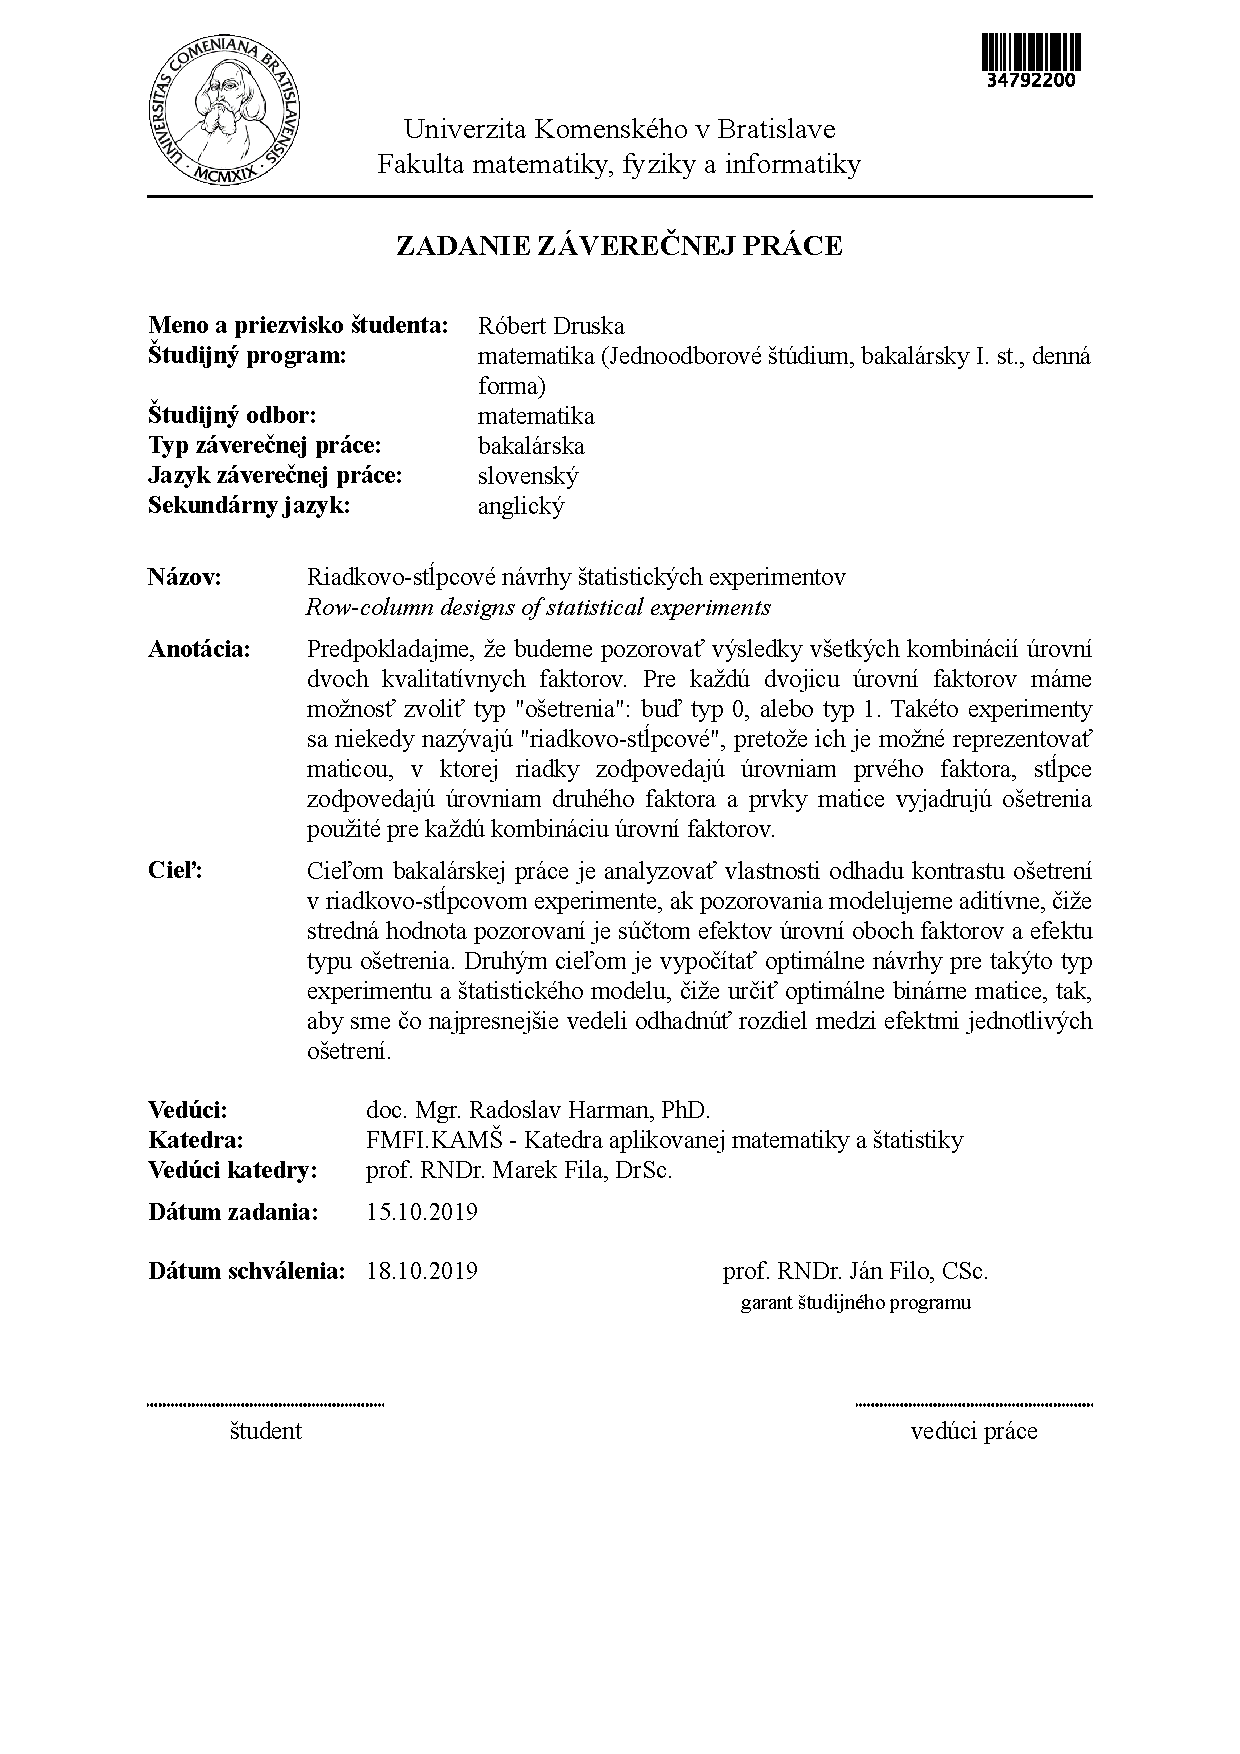
\includepdf[pages={1}, offset=25 -75]{zadanieRD--update.pdf}

  

\vglue0pt
\vfill
\thispagestyle{empty}
\paragraph{Poďakovanie}
TODO


  \newpage
  \thispagestyle{empty}
\section*{Abstrakt}
TODO

\begin{flushleft}
  \textbf{Kľúčové slová:} lineárny regresný model
\end{flushleft}

  \newpage
  \thispagestyle{empty}
\section*{Abstract}
DRUSKA, Róbert: Row-column designs of statistical experiments [Bachelor thesis],
Comenius University in Bratislava,
Faculty of Mathematics, Physics and Informatics,
Department of Applied Mathematics and Statistics,
supervisor: doc. Mgr. Radoslav Harman, PhD.,
Bratislava, 2020, 38 p.

TODO

\begin{flushleft}
  \textbf{Keywords:} linear regression
\end{flushleft}
  \newpage \tableofcontents
  \setcounter{page}{7}
 % \newpage
 % \listoffigures
 % \newpage
 % \listoftables  
  \newpage

    \section*{Úvod}	          
    \markboth{ÚVOD}{ÚVOD}  
    \addcontentsline{toc}{section}{Úvod}
    
    Vykonávanie experimentov a prieskumov patrí medzi populárne mechanizmy, ako potvrdiť či vyvrátiť naše domnienky, alebo odhaliť nové, neočakávané skutočnosti. 
V súčasnosti, vďaka nebývalému rozvoju v oblasti výpočtovej techniky a spracovania dát, je tento trend silnejší, než kedykoľvek v minulosti.

Predtým, než sa experimentátor pustí do zberu dát a ich analýzy, je potrebné experiment navrhnúť tak, aby jeho výsledky dávali dostatočný priestor na 
logickú a nespochybniteľnú analýzu. V ideálnom prípade chceme, aby miera informácie, ktorú zozbierané dáta ponúkajú, bola čo najväčšia.

V našej práci sa budeme zaoberať návrhom tzv. riadkovo-stĺpcových experimentov, v ktorých kombinácie dvoch kvalitatívnych faktorov spájame s jedným z dvoch typov ošetrení. 
Tieto návrhy budeme reprezentovať binárnymi maticami, ktoré, ako ukážeme, vieme transformovať na lineárny regresný model. 
Teóriou lineárnej regresie sa zaoberá množstvo článkov a publikácií, v našej práci budeme čerpať najmä z \cite{pazman, yan}.

Spolu s teóriou lineárnej regresie uvedieme v teoretickej časti niektoré dôležité poznatky z lineárnej algebry, ktoré budeme využívať v celej práci. 
V tretej kapitole v krátkosti opíšeme, ako sme pri našom výskume postupovali.

V štvrtej kapitole budeme skúmať riadkovo-stĺpcové návrhy. Cieľom je analyzovať kontrast medzi dvoma typmi ošetrení. 
Uvedieme, ktorá trieda návrhov ponúka dostatočnú informáciu na odhadnutie tohto kontrastu, a tiež pre ktoré z nich je tento odhad najpresnejší. 
Na záver v krátkosti ukážeme, ako možno riadkovo-stĺpcové návrhy reprezentovať bipartitným grafom. 

  \newpage
  \section{Maticová príprava}
\label{matrix algebra}

V našej práci budeme často pracovať s poznatkami z lineárnej algebry, preto v krátkosti zhrnieme niektoré najdôležitejšie z nich.

\begin{defin}
Nech $A$ je ľubovolná matica typu $m \times n$. Potom symbolom $\mathcal{M}(A)$ označujeme stĺpcový priestor matice $A$, t. j.
\begin{center}
$
\mathcal{M}(A) = \{ Au : u \in \mathbb{R}^n \}
$
\end{center}
Symbolom $\mathcal{K}(A)$ označujeme jadro matice (kernel), t. j.
\begin{center}
$
\mathcal{K}(A) = \{ v \in \mathbb{R}^n : Av = 0 \}
$.
\end{center}
\end{defin}

\begin{lema}
Platí
\begin{center}
$
\mathcal{K}(A) = [\mathcal{M}(A)]^{\perp} \equiv \{ v \in \mathbb{R}^n : {\forall}_{u \in \mathcal{M}(A)} u^T v = 0 \}
$
\end{center}
\end{lema}

\begin{dokaz}


\begin{center}
$
x \in \mathcal{K}(A^T) \Leftrightarrow A^T x = 0 \Leftrightarrow {\forall}_v v^T A^T x = 0 \Leftrightarrow {\forall}_v (Av)^Tx = 0 \Leftrightarrow x \in [\mathcal{M}(A)]^{\perp}
$
\end{center}
\end{dokaz}

\begin{lema}
\label{o stlpcovych priestoroch}
Nech $A$ je ľubovolná matica typu $m \times n$. Potom
\begin{center}
$\mathcal{M}(A^T) = \mathcal{M}(A^T A)$
\end{center}
\end{lema}

\begin{dokaz}
Nech $z \in \mathcal{M}(A^T A)$. Potom existuje také $v$, že $z = A^T A v = A^T u$ pre $u = A v$.
Preto $z \in \mathcal{M}(A^T)$ a teda $\mathcal{M}(A^T A) \subseteq \mathcal{M}(A^T)$.

Teraz nech $z \in \mathcal{K}(A^T A)$. Potom:

\begin{center}
$
A^T A z = (0, 0, \ldots, 0)^T \Rightarrow z^T A^T A z = 0 = (Az)^T Az = ||Az|| \Rightarrow Az = 0
$
\end{center}

Preto $z \in \mathcal{K}(A)$, a teda $\mathcal{K}(A^T A) \subseteq \mathcal{K}(A)$.
Z lineárnej algebry ale vieme, že nulový priestor matice je kolmý doplnok jej riadkového priestoru,
preto predošlý výraz vieme rozšíriť:
\begin{center}
$
[\mathcal{M}(A^T A)]^{\perp} = \mathcal{K}(A^T A) \subseteq \mathcal{K}(A) = [\mathcal{M}(A^T)]^{\perp}
$
\end{center}

Odstránením $\perp$ sa inklúzia obráti, čo spolu s opačnou inklúziou vyššie dáva výsledok $\mathcal{M}(A^T) = \mathcal{M}(A^T A)$.
\end{dokaz}

\begin{defin}
Nech $A$ je ľubovoľná matica. Potom matica $A^-$ taká, že
\begin{center}
$A A^- A = A$
\end{center}
sa nazýva $g$-inverzia (alebo pseudoinverzia) matice $A$.
\end{defin}

\begin{com}
Ak $A^{-1}$ neexistuje, tak pre maticu $A$ existuje nekonečný počet $g$-inverzií.
\end{com}

Pseudoinverzie použijeme neskôr v našej práci, keď budeme skúmať, 
či vektor patrí do stĺpcového priestoru matice. Na to nám poslúži nasledovná veta.

\begin{theorem}
\label{veta3}
Nech rovnica $Ax = y$ má riešenie a nech $A^-$ je ľubovolná $g$-inverzia. Potom $A^- y$ je riešením tejto rovnice.
\end{theorem}

\begin{dokaz}
Keďže $Ax = y$ má riešenie, tak existuje také $x_0$, že $A x_0 = y$. Potom 
\begin{center}
$A (A^- y) = A(A^- A x_0) = A x_0 = y$
\end{center}
\end{dokaz}

  \newpage  
	\section{Riadkovo-stĺpcový aditívny model s dvoma typmi ošetrení}
\label{my model}

Cieľom tejto práce je skúmať experiment reprezentovaný binárnou maticou.
Možná reprezentácia nášho modelu pri matici rozmeru $m \times n$ je takáto:

Uvažujeme model s dvomi kvalitatívnymi faktormi $A$ a $B$, 
pričom faktor $A$ má $m$ úrovní a faktor $B$ $n$ úrovní. 
Pre každú kombináciu faktorov experimentátor zvolí jedno z dvojice ošetrení (angl. treatment).
Budeme uvažovať len aditívny model bez interakcií.

Napríklad faktor $A$ môže označovať dobrovoľníka (t.j. máme $m$ dobrovoľníkov) 
a faktor $B$ účinnú látku, ktorú nazveme liečivo (t.j. máme $n$ liečiv). 
Ošetrenie $0$ reprezentuje podanie liečiva orálnym spôsobom a ošetrenie $1$ vnútrožilne).
Účinok, ktorý po čase nameriame na dobrovoľníkovi, 
závisí aditívne od efektu samotného dobrovoľníka (jeho predispozícií), 
efektu liečiva a efektu ošetrenia. 
Všetky tieto efekty uvažujeme ako neznáme parametere modelu.

Návrh teda možno reprezentovať binárnou maticou 
(alebo bipartitným grafom, čo opíšeme neskoršie vnašej práci).

Cieľom experimentu je odhadnúť rozdiel medzi dvoma efektmi (treamentami).
Cieľom hľadania optimálneho modelu je nájsť taký návrh, pri ktorom
rozptyl Gauss-Markovovho odhadu rozdielu medzi efektmi dvojice ošetrení (t.j. odhadu kontrastu ošetrení) bude čo najmenší.
(Použijeme pri tom Gaussovu-Markovovu vetu z predošlej kapitoly.)

Pre maticu typu $m \times n$ dostaneme teda $mn$ vzťahov tvaru:

\begin{center}
$
y_{ij} = a_i + b_j + t + e_{ij}
$
\end{center}

$i = 1, \ldots, m$; $j = 1, \ldots, n$; $t$ je $t_0$ alebo $t_1$ podľa hodnoty na $ij$-tej pozícii matice a $e_{ij}$ je chyba.
Budeme odhadovať rozdiel medzi $t_0$ a $t_1$.

Z návrhu modelu v podobe binárnej matice tvaru $m \times n$ vytvoríme lineárny regresný model
s maticou tvaru $mn \times (m + n + 2)$, pretože máme $mn$ meraní závislých od $m + n + 2$ premenných.

Príklad:

Maticu návrhu experimentu

\begin{align}
\label{model matrix}
\begin{bmatrix}
1 & 0 & 1 \\
0 & 1 & 0 \\
1 & 0 & 1
\end{bmatrix}
\end{align}

prepíšeme ako:

\begin{align}
\label{linear regression matrix}
\begin{bmatrix}
1 & 0 & 0 & 1 & 0 & 0 & 1 & 0 \\
1 & 0 & 0 & 0 & 1 & 0 & 0 & 1 \\
1 & 0 & 0 & 0 & 0 & 1 & 1 & 0 \\
0 & 1 & 0 & 1 & 0 & 0 & 0 & 1 \\
0 & 1 & 0 & 0 & 1 & 0 & 1 & 0 \\
0 & 1 & 0 & 0 & 0 & 1 & 0 & 1 \\
0 & 0 & 1 & 1 & 0 & 0 & 1 & 0 \\
0 & 0 & 1 & 0 & 1 & 0 & 0 & 1 \\
0 & 0 & 1 & 0 & 0 & 1 & 1 & 0
\end{bmatrix}
\end{align}

Ako presne sme pri generovaní matice postupovali?
Každý riadok reprezentuje jednu z hodnôt v matici (\ref{model matrix}), preto máme dokopy $3 \times 3 = 9$ riadkov.
Prvé tri stĺpce reprezentujú riadok, v ktorom sa hodnota nachádza, ďalšie tri reprezentujú stĺpec.
Vo všeocenosti $ij$-tu pozíciu matice typu $m \times n$ reprezentuje riadok,
ktorý má jednotky na $i$-tej a $(m + j)$-tej pozícii.
Posledné dva stĺpce sú určené tým, či je hodnota $0$ alebo $1$.

Označme vo všeobecnosti maticu modelu (\ref{model matrix}) $B$ a maticu lineárneho zobrazenia (\ref{linear regression matrix}) $X$. 
Predpokladáme lineárne vzťahy, preto dostávame lineárnu regresiu

\begin{center}
$
y = X b + e
$
\end{center}

kde $y$ je vektor dát nameraných v experimente, $b$ je vektor neznámych koeficientov a 
$e = (e_{11}, e_{12}, e_{13}, \ldots, e_{m1}, \dots, e_{mn})^T$ je vektor chýb merania. 
Uvedomme si, že v našej práci nebudeme pracovať s konkrétnym vektorom $y$; 
snažíme sa totiž navrhnúť maticu modelu $B$ (a z nej vyplývajúcu maticu $X$) ešte pred tým, než experiment vykonáme.

Naším cieľom teraz bude odhadnúť rozdiel medzi efektmi $t_0$ a $t_1$, resp. zistiť, 
aká môže byť disperzia tohto odhadu pri danej matici návrhu $B$. 
Modely, pre ktoré bude možná disperzia najmenšia, budeme považovať za optimálne.

V danej lineárnej regresii $y = X b + e$ teda nebudeme odhadovať celý vektor $b$, 
ale len jeho lineárnu kombináciu $h^T b$, kde $h$ je vektor rozmeru $m + n + 2$, 
ktorý má na $m + n$ miestach $0$ a na zvyšných dvoch miestach $+1$ a $-1$, ktoré zodpovedajú efektom $t_0$ a $t_1$. 
Z algoritmu, ktorým sme z matice návrhu $B$ vytvorili maticu lineárnej regresie $X$, 
vyplýva, že vektor $h$ má tvar $(0, 0, 0, \ldots, +1, -1)^T$.

Na zistenie, či $h^T b$ je odhadnuteľné, použijeme vetu (\ref{veta1}), 
a na následné nájdenie minimálneho rozptylu Gauss-Markovovho odhadu rozdielu medzi efektmi 
použijeme Gaussovu-Markovovu vetu (\ref{gauss-markov}).

\subsection{Odhadnuteľnosť $h^T b$}

Pokúsime sa preskúmať, kedy matica návrhu umožňuje odhadnuteľnosť hodnoty $h^T b$ pre vyššie spomenuté $h$. 
Situáciu preskúmame do rozmeru $4 \times 5$ a na základe našich zistení vyslovíme hypotézu pre všeobecný prípad $m \times n$.

Postupovať budeme nasledovne: vyberieme si malý rozmer a pre všetky matice daného rozmeru zistíme, 
či $h^T b$ bude alebo nebude odhadnuteľné, a to nasledovným spôsobom. 
Z danej matice návrhu $B$ vytvoríme maticu lineárnej regresie $X$ spôsobom spomenutým vyššie. 
Hodnota $h^T b$ bude na základe vety (\ref{veta1}) odhadnuteľná práve vtedy, 
keď vektor $h = (0, 0, 0, \ldots, +1, -1)^T$ patrí do stĺpcového priestoru matice $X^T X$.

Označme $M = X^T X$, túto maticu budeme nazývať informačnou maticou. 
Ak $h$ patrí do stĺpcového priestoru $M$, potom existuje taký vektor $v$, že $M v = h$. 
Na základe vety (\ref{veta3}) vieme, že ak toto riešenie existuje, tak sa rovná $M^- h$, pričom zvolená $g$-inverzia môže byť ľubovoľná.
Preto na zistenie, či $h$ patrí do stĺpcového priestoru $M = X^T X$ stačí overiť platnosť rovnosti $M(M^- h) = h$. 

Demonštrujme algoritmus na maticiach rozmeru $3 \times 3$. Existuje $2^9 = 512$ binárnych matíc typu $3 \times 3$, 
a keď sme na nich rozbehli daný algoritmus, dospeli sme k zisteniu, že pri $12$ z nich hodnota $h^T b$ NIE JE odhadnuteľná.
To znamená, že optimálne matice návrhu budeme hľadať v zvyšných $500$ maticiach.

Ako vyzerajú matice, pri ktorých $h^T b$ nie je odhadnuteľné? Zoznam všetkých sa nachádza v Prílohe A, tu uvedieme $3$ z nich:

\begin{center}
$
\begin{bmatrix}
1 & 1 & 1 \\
0 & 0 & 0 \\
1 & 1 & 1 \\
\end{bmatrix}
$, 
$
\begin{bmatrix}
0 & 0 & 1 \\
0 & 0 & 1 \\
0 & 0 & 1 \\
\end{bmatrix}
$, 
$
\begin{bmatrix}
0 & 0 & 0 \\
0 & 0 & 0 \\
0 & 0 & 0 \\
\end{bmatrix}
$
\end{center}

Týmto spôsobom sme pri našom výskume získali zoznam matíc, pri ktorých $h^T b$ nie je odhadnuteľné, až do rozmeru $4 \times 5$.
Zoznam všetkých sa nachádza v GitHub repozitári spomenutom v úvode. 
Na základe podobnosti matíc daného typu sme prišli s nasledovnou hypotézou.

\begin{prop}
\label{statement 1}
$h^T b$ je odhadnuteľné práve vtedy, keď v matici návrhu $B$ existuje aspoň jeden riadok a aspoň jeden stĺpec taký,
ktorý má aspoň jednu $0$ a aspoň jednu $1$.
\end{prop}

\begin{dokaz}
Na základe vety (\ref{veta1}) vieme, že $h^T b$ je odhadnuteľné práve vtedy, keď $h \in \mathcal{M}(X^T)$
(keď $h$ patrí do riadkového priestoru $X$),
preto s danými podmienkami môžeme pracovať ekvivalentne.

$\boxed{\implies}$ Nech $h = (0, \ldots, +1, -1) \in \mathcal{M}(X^T)$. Použijeme dôkaz sporom. 
Nech v matici $B$ typu $m \times n$ neexistuje taký riadok, ktorý má aspoň jednu $0$ a aspoň jednu $1$,
t. j všetky riadky obsahujú buď samé $0$ alebo samé $1$.
Ako vyzerá matica $X$?

Pozrime sa na riadky matice $X$ zodpovedajúce prvému riadku matice $B$.
Sú to práve tie riadky, ktoré majú na prvej pozícii $1$, pričom si uvedomme, že všetky ostatné riadky majú na prvej pozícii $0$.

% TODO
\begin{center}
$
x_1 = (1, 0, \ldots, 1, 0, \ldots, 0, 1, 0)
$,
\end{center}
\begin{center}
$
x_2 = (1, 0, \ldots, 0, 1, \ldots, 0, 1, 0)
$,
\end{center}
\begin{center}
$\vdots$
\end{center}
\begin{center}
$
x_n = (1, 0, \ldots, 0, 0, \ldots, 1, 1, 0)
$
\end{center}

Keďže $h \in \mathcal{M}(X^T)$, existuje taká lineárna kombinácia riadkov $X$, ktorá dokopy dáva vektor $h$.
Aké môžu mať v tejto lineárnej kombinácii zastúpenie riadky $x_1$, ..., $x_n$?
Označme postupne $a_1$, ..., $a_n$ koeficienty vektorov $x_1$, ..., $x_n$ v lineárnej kombinácii riadkov $X$, ktorá dáva vektor $h$.
Keďže $x_1$, ..., $x_n$ sú jediné riadky matice $X$ s $1$ na prvej pozícii a vektor $h$ má na prvej pozícii $0$,
musí platiť $\sum_{i = 1}^n a_i = 0$.

Z predpokladu, že každý z riadkov matice $B$ obsahuje buď samé $0$ alebo samé $1$, vyplýva,
že každý z vektorov $x_1$, ..., $x_n$ má rovnaké posledné dve hodnoty, a to buď $(0, 1)$ alebo $(1, 0)$.
Z toho spolu s rovnosťou $\sum_{i = 1}^n a_i = 0$ vyplýva, že lineárna kombinácia $\sum_{i = 1}^n a_i x_i$
bude mať na posledných dvoch miestach hodnoty $(0, 0)$, a teda nijako "neprispeje" do vektoru $h$.
Vektor $h$ teda nemožno napísať ako lineárnu kombináciu riadkov $X$, čo je podmienka odhadnuteľnosti.

Analogicky môžeme postupovať pre všetky riadky matice $B$.
Týmto spôsobom pokryjeme všetky riadky matice $X$, vďaka čomu dospejeme k záveru,
že z riadkov $X$ nie je možné lineárnou kombináciou zostrojiť vektor $h$.
To nám dáva spor s predpokladom $h \in \mathcal{M}(X^T)$.
Preto nemôže platiť, že všetky riadky matice $B$ obsahujú buď samé $0$ alebo samé $1$,
a platí opačné tvdenie, t.j v $B$ existuje aspoň jeden riadok taký, ktorý obsahuje $0$ aj $1$.

Rovnakou úvahou pre stĺpce $B$ dospejeme k záveru,
že $B$ musí takisto obsahovať aspoň jeden stĺpec obsahujúci $0$ aj $1$.

$\boxed{\impliedby}$ Nech matica $B$ je taká, že existuje aspoň jeden riadok a aspoň jeden stĺpec také, že majú $0$ aj $1$.
Zostrojíme takú lineárnu kombináciu riadkov $X$, ktorá sa bude rovnať $h$.

Nech riadok, ktorý má $0$ aj $1$, je $i$-ty v poradí a stĺpec s rovnakou vlastnosťou je $j$-ty v poradí.
Bez ujmy na všeobecnosti, nech na $ij$-tom mieste matice $B$ sa nachádza $0$, teda $B_{ij} = 0$.

Potom v $i$-tom riadku $B$ sa určite nachádza hodnota $B_{ik} = 1$ a v $j$-tom stĺpci sa nachádza hodnota $B_{lj} = 1$,
pričom, samozrejme, $k \neq j$ a $l \neq i$.
Označme $x_{ij}, x_{ik}, x_{lj}, x_{lk}$ riadky matice $X$ prislúchajúce prvkom $B_{ij}, B_{ik}, B_{lj}, B_{lk}$ matice $B$. Potom:

\begin{center}
$
x_{ij} - x_{ik} - x_{lj} + x_{lk} = (0, 0, 0, \ldots, 0, N_1, N_2)
$
\end{center}
je vektor, ktorý má na prvých $m + n$ miestach $0$, a na posledných dvoch hodnoty $N_1$ a $N_2$, ktoré zatiaľ necháme bokom.
Prečo má daný vektor na prvých $m + n$ miestach $0$?
Vo všeobecnosti má riadok $x_{rs}$ matice $X$ prislúchajúci prvku $B_{rs}$ matice $B$ na prvých $m + n$ miestach dve $1$,
jednu prislúchajúcu riadku, druhú stĺpcu matice $B$. Konkrétne, riadok $x_{rs}$ má $1$ na $r$-tom mieste a $(m + s)$-tom mieste.

Súčet $x_{ij} + x_{lk}$ má teda štyri jednotky na miestach $i, j, m + j, m + k$.
Súčet $x_{ik} + x_{lj}$ má jednotky na tých istých miestach, 
preto $x_{ij} - x_{ik} - x_{lj} + x_{lk} = x_{ij} + x_{lk} - (x_{ik} + x_{lj})$ má na prvých $m + n$ miestach $0$.

Takto to vyzerá, keď zanedbáme stĺpce so samými nulami:
\[
\begin{split}
+(1, 0, 1, 0) \\
-(1, 0, 0, 1) \\
-(0, 1, 1, 0) \\
+(0, 1, 0, 1) \\
=(0, 0, 0, 0) \\
\end{split}
\]

Ako vyzerá chvost $(N_1, N_2)$? Keďže $B_{ij} = 0$ a $B_{ik} = B_{lj} = 1$,
výraz $x_{ij} - x_{ik} - x_{lj}$ nám vytvorí chvost $(1, -2)$ (prípadne $(-2, 1)$, na tom ale nezáleží).
Potom na základe toho, či na mieste $B_{lk}$ matice návrhu bola $0$ alebo $1$,
nám výraz $x_{ij} - x_{ik} - x_{lj} + x_{lk}$ dá na posledných dvoch miestach $(2, -2)$ alebo $(1, -1)$.
Vo všetkých prípadoch vektor $h$ dostaneme ihneď, prípadne po prenásobení konštantou.
Našli sme teda lineárnu kombináciu riadkov $X$, ktorá nám dala vektor $h$, preto $h \in \mathcal{M}(X^T)$. $\square$

\end{dokaz}

\subsection{Ekvivalencie binárnych matíc}

Pre rozmer $m \times n$ existuje $2^{mn}$ binárnych matíc, čo je obrovské číslo už pre malé hodnoty $m$ a $n$.
(Napríklad už pre rozmer $5 \times 5$ máme viac než milión matíc.)
Pre skúmanie špecifík jednotlivých matíc je výhodné uvedomiť si niektoré očividné ekvivalencie medzi maticami, 
čo nám môže výrazne zredukovať počet matíc, s ktorými pracujeme,
 a v konečnom dôsledku nám to umožní pracovať spôsobom “brute force” do väčšieho rozmeru.

\begin{hypoteza}

Matice, ktoré možno spermutovať jednu na druhú riadkovými a stĺpcovými permutáciami, sú ekvivalentné v zmysle, 
že majú rovnakú hodnotu minimálneho rozptylu Gaussovho-Markovho rozdielu medzi dvoma efektmi.

\end{hypoteza}

Hypotézu uvádzame bez matematického dôkazu, ukážeme však, že ak naša interpretácia modelu reprezentovaného binárnou maticou je správna,
hypotéza musí platíť. Model sme interpretovali ako zoznam trojíc pacient, lekár, spôsob prijatia lieku, 
pričom pacienti zodpovedali riadkom, lekári stĺpcom, a spôsob prijatia lieku hodnotám v matici. 
Uvedomme si, že o lekároch ani pacientoch pri výpočte rozptylu nič nevieme. 
Permutáciám riadkov a stĺpcov preto zodpovedá akési „prelabelovanie“ jednotlivých lekárov a pacientov, 
vôbec to ale nezmení štruktúru experimentu. Pripomeňme si, že rozptyl Gaussovho-Markovho rozdielu medzi efektmi 
počítame pred vykonaním experimentu a nameraním dát.

Táto jediná ekvivalencia nám výrazne zredukuje počet matíc, s ktorými musíme počítať. 
V tabuľke uvádzame počet neekvivalentných tried pre štvorcové rozmery až do $6 \times 6$.

\begin{center}
\begin{tabular}{ |c|c|c|c|c|c|c| }
  \hline
  Rozmer & $1 \times 1$ & $2 \times 2$ & $3 \times 3$ & $4 \times 4$ & $5 \times 5$ & $6 \times 6$ \\ \hline
  Počet binárnych matíc & 2 & 16 & 512 & 65 536 & 33 554 432 & 68 719 476 736 \\ \hline
  Počet neekvivalentných tried & 2 & 7 & 36 & 317 & 5 624 & 251 610 \\ \hline
\end{tabular}
\end{center}

\subsection{Optimálnosť návrhu modelu}

Teraz sa pokúsime nájsť modely, ktoré pre nás budú v určitom zmysle optimálne. 
Najprv ale definujme, čo presne optimalita modelu znamená.

\begin{defin}
\label{optimal matrix definition}
Binárnu maticu $B$ návrhu modelu, $B \in \mathbb{R}^{m \times n}$, nazývame optimálnou, 
ak pre všetky binárne matice $C \in \mathbb{R}^{m \times n}$ platí:

\begin{center}
\label{optimal matrix}
$h^T M_{B}^- h \leq h^T M_{C}^- h$
\end{center}
kde $h = (0, 0,\ldots , +1, -1)$ je vektor zodpovedajú lineárnej kombinácii dvoch efektov, 
$M_B$ a $M_C$ sú informačné matice prislúchajúce návrhom $B$, $C$ a $M_{B}^-$, $M_{C}^-$ sú ich ľubovolné pseudoinverzie.

\end{defin}

Nájsť optimálne matice v zmysle definície (\ref{optimal matrix}) je cieľom tejto práce. 
Podobne ako pri skúmaní, či hodnotu $h^T b$ vôbec budeme môcť odhadnúť, 
preskúmame najprv matice malého rozmeru a na základe výsledkov vyslovíme hypotézu pre všeobecný rozmer.

Postupovať budeme nasledovne: zoberieme si malý rozmer a pre všetky binárne matice tohto rozmeru spočítame hodnotu $h^T M^- h$, 
pokiaľ je to možné (viď tvrdenie (\ref{statement 1})). Z množiny týchto hodnôt vyberieme minimum. 
Optimálne návrhy budú tie, ktorých prislúchajúca hodnota bude práve toto minimum.

Optimálne návrhy sme určili do rozmeru $6 \times 5$, tu sú niektoré z nich pre štvorcové rozmery:

\begin{center}
$
\begin{bmatrix}
0 & 1 & 1 \\ 
1 & 0 & 1 \\ 
1 & 1 & 0 \\ 
\end{bmatrix}
$, 
$
\begin{bmatrix}
0 & 0 & 1 & 1 \\
0 & 0 & 1 & 1 \\
1 & 1 & 0 & 0 \\
1 & 1 & 0 & 0 \\
\end{bmatrix}
$, 
$
\begin{bmatrix}
0 & 0 & 1 & 1 & 0 \\
0 & 1 & 0 & 1 & 0 \\
0 & 1 & 1 & 0 & 0 \\
1 & 0 & 0 & 0 & 1 \\
1 & 0 & 0 & 0 & 1 \\
\end{bmatrix}
$
\end{center}

Ďalšie matice sa nachádzajú v prílohe B. Na základe týchto návrhov sme pre štvorcové matice prišli s nasledovnou hypotézou.

\begin{hypoteza}
\label{hypoteza1}
(pre štvorcové matice)

Binárna matica návrhu $B$ rozmeru $2k \times 2k$ je optimálna v zmysle definície (\ref{optimal matrix}) práve vtedy, 
keď má v každom riadku a v každom stĺpci práve $k$ jednotiek (a práve $k$ núl).

Binárna matica návrhu $B$ rozmeru $(2k + 1) \times (2k + 1)$ je optimálna práve vtedy, 
keď všetky jej riadky aj stĺpce majú rovnaký počet jednotiek, a ten počet je buď $k$ alebo $k + 1$.
\end{hypoteza}

Ako to vyzerá pre matice iného, ako štvorcového rozmeru? 
Kľúčový je pomer jednotiek a núl v matici návrhu. 
Všimnime si, že pri štvorcových rozmeroch v predošlej hypotéze je v prípade párneho rozmeru rovnaký počet jednotiek a núl, 
no v prípade nepárneho rozmeru pomer nielenže nie je pol na pol (čo ani nemôže byť), 
ale dokonca k tomuto pomeru ani nie je tak blízko, ako by mohol byť. 
Napríklad pri rozmere $5 \times 5$ by sme mohli očakávať, že pomer jednotiek a núl v optimálnom návrhu bude $13:12$, 
ale podľa hypotézy je to $15:10$. Skutočnosť, že $5$ delí $10$ aj $15$, nie je náhodná, 
a bude zohrávať kľúčovú rolu pri hypotéze o návrhoch iných ako štvorcových rozmerov.

\begin{hypoteza}
\label{hypoteza2}
(pre neštvorcové matice)

Postačujúcou podmienkou optimality pre rozmer $2k \times 2l$ je, ak má matica práve $2kl$ jednotiek a $2kl$ núl, 
pričom v každom z $2k$ riadkov je $l$ jednotiek a $l$ núl a v každom z $2l$ stĺpcov je práve $k$ jednotiek a $k$ núl.

Postačujúcou podmienkou optimality pre rozmer $2k \times 2l + 1$ je, ak má matica práve $(2l + 1)k$ jednotiek a $(2l + 1)k$ núl, 
pričom v každom z $2l + 1$ stĺpcov je práve $k$ jednotiek a $k$ núl, v $k$ riadkoch je $l + 1$ jednotiek a $l$ núl 
a v $k$ zvyšných riadkoch je $l$ jednotiek a $l + 1$ núl.

Ďalej nech bez ujmy na všeobecnosti $k < l$.

Postačujúcou podmienkou optimality pre rozmer $2k + 1 \times 2l + 1$ je, 
ak má matica $(l + 1)(2k + 1)$ jednotiek a $l(2k + 1)$ núl (alebo naopak), 
pričom v každom z $2k + 1$ riadkov je práve $l + 1$ jednotiek a $l$ núl, v $l + k + 1$ stĺpcoch je práve $k + 1$
jednotiek a v $l - k$ stĺpcoch je práve $k$ jednotiek.
\end{hypoteza}

\begin{com}
Podmienky nie sú nutné, pretože napr. pri rozmere $3 \times 6$ sme našli optimálne matice s pomerom jednotiek a núl
nielen $9:9$ (spĺňajúce hypotézu), ale aj $6:12$, čo naznačuje, 
že v niektorých prípadoch matice pokryté hypotézou nie sú všetky optimálne matice daného rozmeru. 
Hypotéza je napriek tomu cenná, pretože pre prax nám poskytuje mechanizmus, ako vytvoriť optimálny návrh experimentu.
\end{com}

Niektoré z optimálnych návrhov pre neštvorcové rozmery:

\begin{center}
$
\begin{bmatrix}
0 & 0 & 1 & 1 \\
0 & 0 & 1 & 1 \\
1 & 1 & 0 & 0 \\
\end{bmatrix}
$,
$
\begin{bmatrix}
0 & 0 & 0 & 0 & 1 & 1 & 1 \\
0 & 1 & 1 & 1 & 0 & 0 & 0 \\
1 & 0 & 0 & 1 & 0 & 0 & 1 \\
\end{bmatrix}
$,
$
\begin{bmatrix}
0 & 0 & 1 & 1 & 1 \\ 
0 & 1 & 0 & 0 & 1 \\ 
0 & 1 & 0 & 1 & 0 \\ 
1 & 0 & 0 & 0 & 1 \\ 
1 & 0 & 1 & 1 & 0 \\ 
1 & 1 & 1 & 0 & 0 \\ 
\end{bmatrix}
$
\end{center}

Niektoré z optimálnych návrhov pre rozmer $3 \times 6$:

\begin{center}
$
\begin{bmatrix}
0 & 0 & 0 & 0 & 1 & 1 \\
0 & 0 & 1 & 1 & 0 & 0 \\
1 & 1 & 0 & 0 & 0 & 0 \\
\end{bmatrix}
$,
$
\begin{bmatrix}
0 & 0 & 0 & 1 & 1 & 1 \\
0 & 0 & 0 & 1 & 1 & 1 \\
1 & 1 & 1 & 0 & 0 & 0 \\
\end{bmatrix}
$,
$
\begin{bmatrix}
0 & 0 & 1 & 1 & 1 & 1 \\
1 & 1 & 0 & 0 & 1 & 1 \\
1 & 1 & 1 & 1 & 0 & 0 \\
\end{bmatrix}
$
\end{center}

\subsection{Hodnota minimálneho rozptylu}

Ako závisí hodnota (minimálna) Gaussovho-Markovovho rozptylu od rozmeru matice návrhu? 
Ukážeme, že minimálny rozptyl má so stúpajúcim rozmerom klesajúcu tendenciu. 
(Čo, napokon, dáva zmysel, pretože väčší rozdiel nám ponúka viac dát na určenie rozdielu medzi dvoma efektmi.)

Hodnoty pre jednotlivé rozmery určíme tak, že pre každý rozmer zoberieme jednu maticu optimálnu 
v zmysle definície (\ref{optimal matrix definition}) a určíme ju pre ňu.

Matice vytvoríme tak, aby spĺňali hypotézu (\ref{hypoteza1}), a to nasledovne.

Pre párny rozmer $2k \times 2k$ rozdelíme maticu na $4$ bloky $k \times k$, 
z nich ľavý horný a pravý dolný budú samé jednotky, zvyšné dva samé nuly. 
Pre nepárny rozmer $(2k + 1) \times (2k + 1)$ budú ľavý horný blok $k \times k$ tvoriť samé jednotky 
a pravý dolný blok $(k + 1) \times (k + 1)$ bude identita, v ktorej sa zamenili jednotky a nuly.

Názorný príklad, ako to vyzerá pre rozmery $6 \times 6$ a $7 \times 7$:

\begin{center}
$
\begin{bmatrix}
1 & 1 & 1 & 0 & 0 & 0 \\
1 & 1 & 1 & 0 & 0 & 0 \\
1 & 1 & 1 & 0 & 0 & 0 \\
0 & 0 & 0 & 1 & 1 & 1 \\
0 & 0 & 0 & 1 & 1 & 1 \\
0 & 0 & 0 & 1 & 1 & 1 \\
\end{bmatrix}
$,
$
\begin{bmatrix}
1 & 1 & 1 & 0 & 0 & 0 & 0 \\
1 & 1 & 1 & 0 & 0 & 0 & 0 \\
1 & 1 & 1 & 0 & 0 & 0 & 0 \\
0 & 0 & 0 & 0 & 1 & 1 & 1 \\
0 & 0 & 0 & 1 & 0 & 1 & 1 \\
0 & 0 & 0 & 1 & 1 & 0 & 1 \\
0 & 0 & 0 & 1 & 1 & 1 & 0 \\
\end{bmatrix}
$
\end{center}

V tabuľke a grafe sú znázornené hodnoty rozptylu do rozmeru $15 \times 15$.

\begin{center}
\begin{tabular}{ |c|c|}
  \hline
  Rozmer & Minimálna hodnota rozptylu \\ \hline
  $2 \times 2$ & 1 \\ \hline
  $3 \times 3$ & 0.5 \\ \hline
  $4 \times 4$ & 0.25 \\ \hline
  $5 \times 5$ & 0.167 \\ \hline
  $6 \times 6$ & 0.111 \\ \hline
  $7 \times 7$ & 0.083 \\ \hline
  $8 \times 8$ & 0.063 \\ \hline
  $9 \times 9$ & 0.05 \\ \hline
  $10 \times 10$ & 0.04 \\ \hline
  $11 \times 11$ & 0.033 \\ \hline
  $12 \times 12$ & 0.028 \\ \hline
  $13 \times 13$ & 0.024 \\ \hline
  $14 \times 14$ & 0.02 \\ \hline
  $15 \times 15$ & 0.018 \\ \hline
\end{tabular}
\end{center}

\begin{figure}[!h]
  \centering
  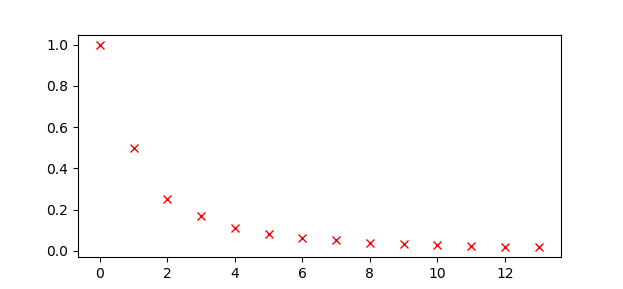
\includegraphics{minimalny_rozptyl.png}
\end{figure}


  \newpage
	\section{Metodika skúmania}

Cieľom nášho skúmania bude nájsť ideálnu maticu vstupu do experimentu (konkrétny problém popíšeme v nasledujúcej kapitole). 
Pokúsime sa vysloviť závery pre všeobecný prípad matice $m \times n$,
avšak pre istý prvotný náhľad do problematiky problém popíšeme a preskúmame na menších rozmeroch, 
konkrétne do rozmeru, do ktorého nám to umožní výpočtová technika. Pracovať budeme s programovacím jazykom \textit{python}.

Od „preskúmania situácie“ do istého rozmeru si sľubujeme dôležité náhľady, 
ktoré nám umožnia vysloviť závery a hypotézy pre všeobecný prípad $m \times n$. 
Tie sa následne pokúsime dokázať matematickými metódami.

Kompletný kód, ktorý sme pri našom výškume použili, sa nachádza v \emph{Github} repozitári na stránke
\url{https://github.com/druskacik/optimal-designs-bachelor-thesis-}.

  \newpage
  \section{Riadkovo-stĺpcový aditívny model s dvoma typmi ošetrení}
\label{my model}

Cieľom tejto práce je skúmať experiment reprezentovaný binárnou maticou.
Možná reprezentácia nášho modelu pri matici rozmeru $m \times n$ je takáto:

Uvažujeme model s dvomi kvalitatívnymi faktormi $A$ a $B$, 
pričom faktor $A$ má $m$ úrovní a faktor $B$ $n$ úrovní. 
Pre každú kombináciu faktorov experimentátor zvolí jedno z dvojice ošetrení (angl. treatment).
Budeme uvažovať len aditívny model bez interakcií.

Napríklad faktor $A$ môže označovať dobrovoľníka (t.j. máme $m$ dobrovoľníkov) 
a faktor $B$ účinnú látku, ktorú nazveme liečivo (t.j. máme $n$ liečiv). 
Ošetrenie $0$ reprezentuje podanie liečiva orálnym spôsobom a ošetrenie $1$ vnútrožilne).
Účinok, ktorý po čase nameriame na dobrovoľníkovi, 
závisí aditívne od efektu samotného dobrovoľníka (jeho predispozícií), 
efektu liečiva a efektu ošetrenia. 
Všetky tieto efekty uvažujeme ako neznáme parametere modelu.

Návrh teda možno reprezentovať binárnou maticou 
(alebo bipartitným grafom, čo opíšeme neskoršie v našej práci).

Cieľom experimentu je odhadnúť rozdiel medzi efektmi daných dvoch ošetrení.
Cieľom hľadania optimálneho modelu je nájsť taký návrh, pri ktorom
rozptyl Gauss-Markovovho odhadu rozdielu medzi efektmi dvojice ošetrení (t.j. odhadu kontrastu ošetrení) bude čo najmenší.

Pre maticu typu $m \times n$ dostaneme teda $mn$ vzťahov tvaru:

\begin{center}
$
y_{ij} = a_i + b_j + t + e_{ij}
$,
\end{center}

$i = 1, \ldots, m$; $j = 1, \ldots, n$; $a_i$ je efekt $i$-tej úrovne faktora $A$ a $b_j$ efekt $j$-tej úrovne faktora $B$; $t$ je $t_0$ alebo $t_1$ podľa hodnoty na $ij$-tej pozícii matice a $e_{ij}$ je chyba.
Budeme odhadovať rozdiel medzi $t_0$ a $t_1$.

Z návrhu modelu v podobe binárnej matice tvaru $m \times n$ vytvoríme lineárny regresný model
s maticou tvaru $mn \times (m + n + 2)$, pretože máme $mn$ meraní závislých od $m + n + 2$ parametrov.

Príklad:

Matica návrhu experimentu

\begin{align}
\label{model matrix}
B =
\begin{bmatrix}
1 & 0 & 1 \\
0 & 1 & 0 \\
1 & 0 & 1
\end{bmatrix}
\end{align}

vedie k matici modelu:

\begin{align}
\label{linear regression matrix}
X =
\begin{bmatrix}
1 & 0 & 0 & 1 & 0 & 0 & 1 & 0 \\
1 & 0 & 0 & 0 & 1 & 0 & 0 & 1 \\
1 & 0 & 0 & 0 & 0 & 1 & 1 & 0 \\
0 & 1 & 0 & 1 & 0 & 0 & 0 & 1 \\
0 & 1 & 0 & 0 & 1 & 0 & 1 & 0 \\
0 & 1 & 0 & 0 & 0 & 1 & 0 & 1 \\
0 & 0 & 1 & 1 & 0 & 0 & 1 & 0 \\
0 & 0 & 1 & 0 & 1 & 0 & 0 & 1 \\
0 & 0 & 1 & 0 & 0 & 1 & 1 & 0
\end{bmatrix}
.
\end{align}

Ako presne sme pri generovaní matice postupovali?
Každý riadok reprezentuje jednu z hodnôt v matici (\ref{model matrix}), preto máme dokopy $3 \times 3 = 9$ riadkov.
Prvé tri stĺpce reprezentujú riadok, v ktorom sa hodnota nachádza, ďalšie tri reprezentujú stĺpec.
Vo všeobecnosti $ij$-tu pozíciu matice typu $m \times n$ reprezentuje riadok,
ktorý má jednotky na $i$-tej a $(m + j)$-tej pozícii.
Posledné dva stĺpce sú určené tým, či je hodnota $0$ alebo $1$.

Predpokladáme lineárne vzťahy, preto dostávame lineárnu regresiu

\begin{center}
$
y = X b + e
$,
\end{center}

kde $y$ je vektor dát nameraných v experimente, $b = (a_1, \ldots, a_m, b_1, \ldots, b_n, t_0, t_1)$ je vektor neznámych koeficientov a 
$e = (e_{11}, e_{12}, e_{13}, \ldots, e_{m1}, \dots, e_{mn})^T$ je vektor chýb merania. 
Uvedomme si, že v našej práci nebudeme pracovať s konkrétnym vektorom $y$; 
snažíme sa totiž navrhnúť maticu návrhu experimentu $B$ (a z nej vyplývajúcu maticu modelu $X$) ešte pred tým, než experiment vykonáme.

Naším cieľom teraz bude odhadnúť rozdiel medzi efektmi $t_0$ a $t_1$, resp. zistiť, 
aká môže byť disperzia tohto odhadu pri danej matici návrhu $B$. 
Modely, pre ktoré bude možná disperzia najmenšia, budeme považovať za optimálne.

V danej lineárnej regresii $y = X b + e$ teda nebudeme odhadovať celý vektor $b$, 
ale len jeho lineárnu kombináciu $h^T b$, kde $h$ je vektor rozmeru $m + n + 2$, 
ktorý má na $m + n$ miestach $0$ a na zvyšných dvoch miestach $+1$ a $-1$, ktoré zodpovedajú efektom $t_0$ a $t_1$. 
Z algoritmu, ktorým sme z matice návrhu $B$ vytvorili maticu lineárnej regresie $X$, 
vyplýva, že vektor $h$ má tvar $(0, 0, 0, \ldots, +1, -1)^T$.

Na zistenie, či $h^T b$ je odhadnuteľné, použijeme vetu (\ref{veta1}), 
a na následné nájdenie minimálneho rozptylu Gauss-Markovovho odhadu rozdielu medzi efektami 
použijeme Gaussovu-Markovovu vetu (\ref{gauss-markov}).

\subsection{Odhadnuteľnosť $h^T b$}

Pokúsime sa preskúmať, kedy matica návrhu umožňuje odhadnuteľnosť hodnoty $h^T b$ pre vyššie spomenuté $h$. 
Situáciu preskúmame do rozmeru $4 \times 5$ a na základe našich zistení vyslovíme hypotézu pre všeobecný prípad $m \times n$.

Postupovať budeme nasledovne: vyberieme si malý rozmer a pre všetky matice daného rozmeru zistíme, 
či $h^T b$ bude alebo nebude odhadnuteľné, a to nasledovným spôsobom. 
Z danej matice návrhu $B$ vytvoríme maticu lineárnej regresie $X$ spôsobom spomenutým vyššie. 
Hodnota $h^T b$ bude na základe vety (\ref{veta1}) odhadnuteľná práve vtedy, 
keď vektor $h = (0, 0, 0, \ldots, +1, -1)^T$ patrí do stĺpcového priestoru matice $X^T X$.

Označme $M = X^T X$, túto maticu budeme nazývať informačnou maticou. 
Ak $h$ patrí do stĺpcového priestoru $M$, potom existuje taký vektor $v$, že $M v = h$. 
Na základe vety (\ref{veta4}) vieme, že ak toto riešenie existuje, tak sa rovná $M^- h$, pričom zvolená $g$-inverzia môže byť ľubovoľná.
Preto na zistenie, či $h$ patrí do stĺpcového priestoru $M = X^T X$ stačí overiť platnosť rovnosti $M(M^- h) = h$. 

Demonštrujme algoritmus na maticiach rozmeru $3 \times 3$. Existuje $2^9 = 512$ binárnych matíc typu $3 \times 3$, 
a keď sme na ne aplikovali daný algoritmus, dospeli sme k zisteniu, že pri $18$ z nich hodnota $h^T b$ \emph{nie je} odhadnuteľná.
To znamená, že optimálne matice návrhu budeme hľadať v zvyšných $492$ maticiach.

Ako vyzerajú matice, pri ktorých $h^T b$ nie je odhadnuteľné? Zoznam všetkých sa nachádza v prílohe \hyperref[appendix:a]{A}, tu uvedieme $3$ z nich:

\begin{center}
$
\begin{bmatrix}
1 & 1 & 1 \\
0 & 0 & 0 \\
1 & 1 & 1 \\
\end{bmatrix}
$, 
$
\begin{bmatrix}
0 & 0 & 1 \\
0 & 0 & 1 \\
0 & 0 & 1 \\
\end{bmatrix}
$, 
$
\begin{bmatrix}
0 & 0 & 0 \\
0 & 0 & 0 \\
0 & 0 & 0 \\
\end{bmatrix}
$.
\end{center}

Týmto spôsobom sme pri našom výskume získali zoznam matíc, pri ktorých $h^T b$ nie je odhadnuteľné, až do rozmeru $4 \times 5$.
Zoznam všetkých sa nachádza v GitHub repozitári spomenutom v úvode. 
Na základe podobnosti matíc daného typu sme odvodili nasledovné tvrdenie.

\begin{prop}
\label{statement 1}
$h^T b$ je odhadnuteľné práve vtedy, keď v matici návrhu $B$ existuje aspoň jeden riadok a aspoň jeden stĺpec taký,
ktorý má aspoň jednu $0$ a aspoň jednu $1$.
\end{prop}

\begin{dokaz}
Na základe vety (\ref{veta1}) vieme, že $h^T b$ je odhadnuteľné práve vtedy, keď $h \in \mathcal{M}(X^T)$
(keď $h$ patrí do riadkového priestoru $X$),
preto s danými podmienkami môžeme pracovať ekvivalentne.

$\boxed{\implies}$ Nech $h = (0, \ldots, 0, +1, -1) \in \mathcal{M}(X^T)$. Použijeme dôkaz sporom. 
Nech v matici $B$ typu $m \times n$ neexistuje taký riadok, ktorý má aspoň jednu $0$ a aspoň jednu $1$,
t. j všetky riadky obsahujú buď samé $0$ alebo samé $1$.
Ako vyzerá matica $X$?

Pozrime sa na riadky matice $X$ zodpovedajúce prvému riadku matice $B$.
Sú to práve tie riadky, ktoré majú na prvej pozícii $1$, pričom si uvedomme, že všetky ostatné riadky majú na prvej pozícii $0$.

% TODO
\begin{center}
$
x_1 = (1, 0, \ldots, 1, 0, \ldots, 0, 1, 0)
$,
\end{center}
\begin{center}
$
x_2 = (1, 0, \ldots, 0, 1, \ldots, 0, 1, 0)
$,
\end{center}
\begin{center}
$\vdots$
\end{center}
\begin{center}
$
x_n = (1, 0, \ldots, 0, 0, \ldots, 1, 1, 0)
$
\end{center}

Keďže $h \in \mathcal{M}(X^T)$, existuje taká lineárna kombinácia riadkov $X$, ktorá dokopy dáva vektor $h$.
Aké môžu mať v tejto lineárnej kombinácii zastúpenie riadky $x_1$, ..., $x_n$?
Označme postupne $a_1$, ..., $a_n$ koeficienty vektorov $x_1$, ..., $x_n$ v lineárnej kombinácii riadkov $X$, ktorá dáva vektor $h$.
Keďže $x_1$, ..., $x_n$ sú jediné riadky matice $X$ s $1$ na prvej pozícii a vektor $h$ má na prvej pozícii $0$,
musí platiť $\sum_{i = 1}^n a_i = 0$.

Z predpokladu, že každý z riadkov matice $B$ obsahuje buď samé $0$ alebo samé $1$, vyplýva,
že každý z vektorov $x_1$, ..., $x_n$ má rovnaké posledné dve hodnoty, a to buď $(0, 1)$ alebo $(1, 0)$.
Z toho spolu s rovnosťou $\sum_{i = 1}^n a_i = 0$ vyplýva, že lineárna kombinácia $\sum_{i = 1}^n a_i x_i$
bude mať na posledných dvoch miestach hodnoty $(0, 0)$, a teda nijako "neprispeje" do vektoru $h$.
Vektor $h$ teda nemožno napísať ako lineárnu kombináciu riadkov $X$, čo je podmienka odhadnuteľnosti.

Analogicky môžeme postupovať pre všetky riadky matice $B$.
Týmto spôsobom pokryjeme všetky riadky matice $X$, vďaka čomu dospejeme k záveru,
že z riadkov $X$ nie je možné lineárnou kombináciou zostrojiť vektor $h$.
To nám dáva spor s predpokladom $h \in \mathcal{M}(X^T)$.
Preto nemôže platiť, že všetky riadky matice $B$ obsahujú buď samé $0$ alebo samé $1$,
a platí opačné tvrdenie, t.j v $B$ existuje aspoň jeden riadok taký, ktorý obsahuje $0$ aj $1$.

Rovnakou úvahou pre stĺpce $B$ dospejeme k záveru,
že $B$ musí takisto obsahovať aspoň jeden stĺpec obsahujúci $0$ aj $1$.

$\boxed{\impliedby}$ Nech matica $B$ je taká, že existuje aspoň jeden riadok a aspoň jeden stĺpec také, že majú $0$ aj $1$.
Zostrojíme takú lineárnu kombináciu riadkov $X$, ktorá sa bude rovnať $h$.

Nech riadok, ktorý má $0$ aj $1$, je $i$-ty v poradí a stĺpec s rovnakou vlastnosťou je $j$-ty v poradí.
Bez ujmy na všeobecnosti, nech na $ij$-tom mieste matice $B$ sa nachádza $0$, teda $B_{ij} = 0$.

Potom v $i$-tom riadku $B$ sa určite nachádza hodnota $B_{ik} = 1$ a v $j$-tom stĺpci sa nachádza hodnota $B_{lj} = 1$,
pričom, samozrejme, $k \neq j$ a $l \neq i$.
Označme $x_{ij}, x_{ik}, x_{lj}, x_{lk}$ riadky matice $X$ prislúchajúce prvkom $B_{ij}, B_{ik}, B_{lj}, B_{lk}$ matice $B$. Potom:

\begin{center}
$
x_{ij} - x_{ik} - x_{lj} + x_{lk} = (0, 0, 0, \ldots, 0, N_1, N_2)
$
\end{center}
je vektor, ktorý má na prvých $m + n$ miestach $0$, a na posledných dvoch hodnoty $N_1$ a $N_2$, ktoré zatiaľ necháme bokom.
Prečo má daný vektor na prvých $m + n$ miestach $0$?
Vo všeobecnosti má riadok $x_{rs}$ matice $X$ prislúchajúci prvku $B_{rs}$ matice $B$ na prvých $m + n$ miestach dve $1$,
jednu prislúchajúcu riadku, druhú stĺpcu matice $B$. Konkrétne, riadok $x_{rs}$ má $1$ na $r$-tom mieste a $(m + s)$-tom mieste.

Súčet $x_{ij} + x_{lk}$ má teda štyri jednotky na miestach $i, j, m + j, m + k$.
Súčet $x_{ik} + x_{lj}$ má jednotky na tých istých miestach, 
preto $x_{ij} - x_{ik} - x_{lj} + x_{lk} = x_{ij} + x_{lk} - (x_{ik} + x_{lj})$ má na prvých $m + n$ miestach $0$.

Takto to vyzerá, keď zanedbáme stĺpce so samými nulami:
\[
\begin{split}
+(1, 0, 1, 0) \\
-(1, 0, 0, 1) \\
-(0, 1, 1, 0) \\
+(0, 1, 0, 1) \\
=(0, 0, 0, 0) \\
\end{split}
.
\]

Ako vyzerá "chvost" $(N_1, N_2)$ vektora $x_{ij} - x_{ik} - x_{lj} + x_{lk}$? Keďže $B_{ij} = 0$ a $B_{ik} = B_{lj} = 1$,
výraz $x_{ij} - x_{ik} - x_{lj}$ nám vytvorí chvost $(1, -2)$ (prípadne $(-2, 1)$, na tom ale nezáleží).
Potom na základe toho, či na mieste $B_{lk}$ matice návrhu bola $0$ alebo $1$,
nám výraz $x_{ij} - x_{ik} - x_{lj} + x_{lk}$ dá na posledných dvoch miestach $(2, -2)$ alebo $(1, -1)$.
Vo všetkých prípadoch vektor $h$ dostaneme ihneď, prípadne po prenásobení konštantou.
Našli sme teda lineárnu kombináciu riadkov $X$, ktorá nám dala vektor $h$, preto $h \in \mathcal{M}(X^T)$. $\square$

\end{dokaz}

Uvedomme si, že toto tvrdenie dáva intuitívne význam. Ak by sme totiž organizovali experiment napr. podľa druhej matice so zoznamu vyššie, 
tak by sme nevedeli rozlíšiť, či sú pozorované rozdiely medzi meraniami zodpovedajúcimi prvým dvom stĺpcom a posledným stĺpcom spôsobené rozdielom medzi efektami ošetrení, 
alebo rozdielom medzi efektami ošetrovateľov 1 a 2 v porovnaní s ošetrovateľom 3.

\subsection{Ekvivalencie binárnych matíc}

Pre rozmer $m \times n$ existuje $2^{mn}$ binárnych matíc, čo je obrovské číslo už pre malé hodnoty $m$ a $n$.
(Napríklad už pre rozmer $5 \times 5$ máme viac než milión matíc.)
Pre skúmanie špecifík jednotlivých matíc je výhodné uvedomiť si niektoré očividné ekvivalencie medzi maticami, 
čo nám môže výrazne zredukovať počet matíc, s ktorými pracujeme,
 a v konečnom dôsledku nám to umožní pracovať spôsobom “brute force” do väčšieho rozmeru.

\begin{hypoteza}

Matice, ktoré možno spermutovať jednu na druhú riadkovými a stĺpcovými permutáciami, sú ekvivalentné v zmysle, 
že majú rovnakú hodnotu minimálneho rozptylu Gaussovho-Markovovho odhadu rozdielu medzi efektami ošetrení.

\end{hypoteza}

Hypotézu uvádzame bez matematického dôkazu, ukážeme však, že ak naša interpretácia modelu reprezentovaného binárnou maticou je správna,
hypotéza musí platíť. Model sme interpretovali ako zoznam trojíc dobrovoľník, liečivo, spôsob jeho prijatia, 
pričom dobrovoľníci zodpovedali riadkom, liečivá stĺpcom, a spôsob prijatia liečiva hodnotám v matici. 
Uvedomme si, že o efektoch dobrovoľníkov ani liečiv pri výpočte rozptylu nič nevieme. 
Permutáciám riadkov a stĺpcov preto zodpovedá akési „preznačenie“ jednotlivých dobrovoľníkov a liečiv, 
vôbec to ale nezmení štruktúru experimentu. Pripomeňme si, že rozptyl Gaussovho-Markovovho odhadu rozdielu medzi efektami
počítame pred vykonaním experimentu a nameraním dát.

Táto jediná ekvivalencia nám výrazne zredukuje počet matíc, s ktorými musíme počítať. 
V tabuľke uvádzame počet neekvivalentných tried pre štvorcové rozmery až do $6 \times 6$.

\begin{center}
\begin{tabular}{ |c|c|c|c|c|c|c| }
  \hline
  Rozmer & $1 \times 1$ & $2 \times 2$ & $3 \times 3$ & $4 \times 4$ & $5 \times 5$ & $6 \times 6$ \\ \hline
  Počet binárnych matíc & 2 & 16 & 512 & 65 536 & 33 554 432 & 68 719 476 736 \\ \hline
  Počet neekvivalentných tried & 2 & 7 & 36 & 317 & 5 624 & 251 610 \\ \hline
\end{tabular}
\end{center}

\subsection{Optimálnosť návrhu experimentu}

Teraz sa pokúsime nájsť modely, ktoré pre nás budú v určitom zmysle optimálne. 
Najprv ale definujme, čo presne optimalita modelu znamená.

\begin{defin}
\label{optimal matrix definition}
Nech $h = (0, 0,\ldots , +1, -1)^T$ je vektor zodpovedajúci lineárnej kombinácii dvoch efektov
a nech $B \in \mathbb{R}^{m \times n}$ je taká binárna matica, že pre jej informačnú maticu $M_B$ platí $h \in \mathcal{M}(M_B)$.
Potom $B$ nazývame optimálnou, ak pre všetky binárne matice $C \in \mathbb{R}^{m \times n}$ také,
že $h \in \mathcal{M}(M_C)$ pre ich informačnú maticu $M_C$, platí:

\begin{center}
\label{optimal matrix}
$h^T M_{B}^- h \leq h^T M_{C}^- h$,
\end{center}
kde $M_{B}^-$ a $M_{C}^-$ sú ľubovoľné $g$-inverzie informačných matíc $M_B$ a $M_C$.

\end{defin}

Nájsť optimálne matice v zmysle definície (\ref{optimal matrix}) je jedným z cieľov tejto práce. 
Podobne ako pri skúmaní, či hodnotu $h^T b$ vôbec budeme môcť odhadnúť, 
preskúmame najprv matice malého rozmeru a na základe výsledkov vyslovíme hypotézu pre všeobecný rozmer.

Postupovať budeme nasledovne: zoberieme si malý rozmer a pre všetky binárne matice tohto rozmeru spočítame hodnotu $h^T M^- h$, 
pokiaľ je to možné (viď tvrdenie (\ref{statement 1})). Z množiny týchto hodnôt vyberieme minimum. 
Optimálne návrhy budú tie, ktorých prislúchajúca hodnota bude práve toto minimum.

Optimálne návrhy sme určili do rozmeru $6 \times 5$, tu sú niektoré z nich pre štvorcové rozmery:

\begin{center}
$
\begin{bmatrix}
0 & 1 & 1 \\ 
1 & 0 & 1 \\ 
1 & 1 & 0 \\ 
\end{bmatrix}
$, 
$
\begin{bmatrix}
0 & 0 & 1 & 1 \\
0 & 0 & 1 & 1 \\
1 & 1 & 0 & 0 \\
1 & 1 & 0 & 0 \\
\end{bmatrix}
$, 
$
\begin{bmatrix}
0 & 0 & 1 & 1 & 0 \\
0 & 1 & 0 & 1 & 0 \\
0 & 1 & 1 & 0 & 0 \\
1 & 0 & 0 & 0 & 1 \\
1 & 0 & 0 & 0 & 1 \\
\end{bmatrix}
$.
\end{center}

Ďalšie matice sa nachádzajú v prílohe \hyperref[appendix:b]{B}. Na základe týchto návrhov sme pre štvorcové matice odvodili nasledovnú hypotézu.

\begin{hypoteza}
\label{hypoteza1}
(pre štvorcové matice)

Binárna matica návrhu $B$ rozmeru $2k \times 2k$ je optimálna v zmysle definície (\ref{optimal matrix}) práve vtedy, 
keď má v každom riadku a v každom stĺpci práve $k$ jednotiek (a práve $k$ núl).

Binárna matica návrhu $B$ rozmeru $(2k + 1) \times (2k + 1)$ je optimálna práve vtedy, 
keď všetky jej riadky aj stĺpce majú rovnaký počet jednotiek, a ten počet je buď $k$ alebo $k + 1$.
\end{hypoteza}

\begin{com}
Hypotéza je do rozmeru $6 \times 6$ tvrdením, pretože sa nám to podarilo ukázať úplnou enumeráciou všetkých možných návrhov.
\end{com}

Ako to vyzerá pre matice iného, ako štvorcového rozmeru? 
Kľúčový je pomer jednotiek a núl v matici návrhu. 
Všimnime si, že pri štvorcových rozmeroch v predošlej hypotéze je v prípade párneho rozmeru rovnaký počet jednotiek a núl, 
no v prípade nepárneho rozmeru pomer nielenže nie je pol na pol (čo ani nemôže byť), 
ale dokonca k tomuto pomeru ani nie je tak blízko, ako by mohol byť. 
Napríklad pri rozmere $5 \times 5$ by sme mohli očakávať, že pomer jednotiek a núl v optimálnom návrhu bude $13:12$, 
ale podľa hypotézy je to $15:10$. Skutočnosť, že $5$ delí $10$ aj $15$, nie je náhodná, 
a bude zohrávať kľúčovú rolu pri hypotéze o návrhoch iných ako štvorcových rozmerov.

\begin{hypoteza}
\label{hypoteza2}
(pre neštvorcové matice)

Postačujúcou podmienkou optimality pre rozmer $2k \times 2l$ je, ak má matica práve $2kl$ jednotiek a $2kl$ núl, 
pričom v každom z $2k$ riadkov je $l$ jednotiek a $l$ núl a v každom z $2l$ stĺpcov je práve $k$ jednotiek a $k$ núl.

Postačujúcou podmienkou optimality pre rozmer $2k \times 2l + 1$ je, ak má matica práve $(2l + 1)k$ jednotiek a $(2l + 1)k$ núl, 
pričom v každom z $2l + 1$ stĺpcov je práve $k$ jednotiek a $k$ núl, v $k$ riadkoch je $l + 1$ jednotiek a $l$ núl 
a v $k$ zvyšných riadkoch je $l$ jednotiek a $l + 1$ núl.

Ďalej nech bez ujmy na všeobecnosti $k < l$.

Postačujúcou podmienkou optimality pre rozmer $(2k + 1) \times (2l + 1)$ je, 
ak má matica $(l + 1)(2k + 1)$ jednotiek a $l(2k + 1)$ núl (alebo naopak), 
pričom v každom z $2k + 1$ riadkov je práve $l + 1$ jednotiek a $l$ núl, v $l + k + 1$ stĺpcoch je práve $k + 1$
jednotiek a v $l - k$ stĺpcoch je práve $k$ jednotiek.
\end{hypoteza}

\begin{com}
Podmienky nie sú nutné, pretože napr. pri rozmere $3 \times 6$ sme našli optimálne matice s pomerom jednotiek a núl
nielen $9:9$ (spĺňajúce hypotézu), ale aj $6:12$, čo dokazuje, 
že v niektorých prípadoch matice pokryté hypotézou nie sú všetky optimálne matice daného rozmeru. 
Hypotéza je napriek tomu cenná, pretože pre prax nám poskytuje mechanizmus, ako vytvoriť optimálny návrh experimentu.
\end{com}

Niektoré z optimálnych návrhov pre neštvorcové rozmery:

\begin{center}
$
\begin{bmatrix}
0 & 0 & 1 & 1 \\
0 & 0 & 1 & 1 \\
1 & 1 & 0 & 0 \\
\end{bmatrix}
$,
$
\begin{bmatrix}
0 & 0 & 0 & 0 & 1 & 1 & 1 \\
0 & 1 & 1 & 1 & 0 & 0 & 0 \\
1 & 0 & 0 & 1 & 0 & 0 & 1 \\
\end{bmatrix}
$,
$
\begin{bmatrix}
0 & 0 & 1 & 1 & 1 \\ 
0 & 1 & 0 & 0 & 1 \\ 
0 & 1 & 0 & 1 & 0 \\ 
1 & 0 & 0 & 0 & 1 \\ 
1 & 0 & 1 & 1 & 0 \\ 
1 & 1 & 1 & 0 & 0 \\ 
\end{bmatrix}
$.
\end{center}

Niektoré z optimálnych návrhov pre rozmer $3 \times 6$:

\begin{center}
$
\begin{bmatrix}
0 & 0 & 0 & 0 & 1 & 1 \\
0 & 0 & 1 & 1 & 0 & 0 \\
1 & 1 & 0 & 0 & 0 & 0 \\
\end{bmatrix}
$,
$
\begin{bmatrix}
0 & 0 & 0 & 1 & 1 & 1 \\
0 & 0 & 0 & 1 & 1 & 1 \\
1 & 1 & 1 & 0 & 0 & 0 \\
\end{bmatrix}
$,
$
\begin{bmatrix}
0 & 0 & 1 & 1 & 1 & 1 \\
1 & 1 & 0 & 0 & 1 & 1 \\
1 & 1 & 1 & 1 & 0 & 0 \\
\end{bmatrix}
$.
\end{center}

Napriek tomu, že hypotézu o optimálnych maticiach sa nám matematicky dokázať nepodarilo, numericky sme až do rozmeru $30 \times 30$ ukázali,
že zmena jednej hodnoty v nami navrhovanom optimálnom návrhu spôsobí zväčšenie hľadaného rozptylu.
Dané matice teda určite tvoria lokálne minimum (na okolí tých matíc, ktoré majú odlišnú najviac jednu hodnotu).

\subsection{Hodnota minimálneho rozptylu}

Ako závisí hodnota Gaussovho-Markovovho odhadu rozdielu medzi efektami od rozmeru matice návrhu? 
Ukážeme, že tento najmenší dosiahnuteľný rozptyl má so stúpajúcim rozmerom klesajúcu tendenciu. 
(Čo, napokon, dáva zmysel, pretože väčší rozdiel nám ponúka viac dát na určenie rozdielu medzi dvoma efektmi.)

Hodnoty pre jednotlivé rozmery určíme tak, že pre každý rozmer zoberieme jednu maticu optimálnu 
v zmysle definície (\ref{optimal matrix definition}).

Pre párny rozmer $2k \times 2k$ rozdelíme maticu na $4$ bloky $k \times k$, 
z nich ľavý horný a pravý dolný budú samé jednotky, zvyšné dva samé nuly. 
Pre nepárny rozmer $(2k + 1) \times (2k + 1)$ budú ľavý horný blok $k \times k$ tvoriť samé jednotky 
a pravý dolný blok $(k + 1) \times (k + 1)$ bude identita, v ktorej sa zamenili jednotky a nuly.

Jednoduchý \emph{python} kód, ktorý generuje optimálnu maticu návrhu experimentu pre ľubovoľný štvorcový rozmer,
sa nachádza v prílohe \hyperref[appendix:d]{D}.

Názorný príklad, ako to vyzerá pre rozmery $6 \times 6$ a $7 \times 7$:

\begin{center}
$
\begin{bmatrix}
1 & 1 & 1 & 0 & 0 & 0 \\
1 & 1 & 1 & 0 & 0 & 0 \\
1 & 1 & 1 & 0 & 0 & 0 \\
0 & 0 & 0 & 1 & 1 & 1 \\
0 & 0 & 0 & 1 & 1 & 1 \\
0 & 0 & 0 & 1 & 1 & 1 \\
\end{bmatrix}
$,
$
\begin{bmatrix}
1 & 1 & 1 & 0 & 0 & 0 & 0 \\
1 & 1 & 1 & 0 & 0 & 0 & 0 \\
1 & 1 & 1 & 0 & 0 & 0 & 0 \\
0 & 0 & 0 & 0 & 1 & 1 & 1 \\
0 & 0 & 0 & 1 & 0 & 1 & 1 \\
0 & 0 & 0 & 1 & 1 & 0 & 1 \\
0 & 0 & 0 & 1 & 1 & 1 & 0 \\
\end{bmatrix}
$.
\end{center}

V tabuľke a grafe sú znázornené hodnoty rozptylu do rozmeru $15 \times 15$.

\begin{center}
\begin{tabular}{ |c|c|}
  \hline
  Rozmer & Minimálna hodnota rozptylu \\ \hline
  $2 \times 2$ & 1 \\ \hline
  $3 \times 3$ & 0.5 \\ \hline
  $4 \times 4$ & 0.25 \\ \hline
  $5 \times 5$ & 0.167 \\ \hline
  $6 \times 6$ & 0.111 \\ \hline
  $7 \times 7$ & 0.083 \\ \hline
  $8 \times 8$ & 0.063 \\ \hline
  $9 \times 9$ & 0.05 \\ \hline
  $10 \times 10$ & 0.04 \\ \hline
  $11 \times 11$ & 0.033 \\ \hline
  $12 \times 12$ & 0.028 \\ \hline
  $13 \times 13$ & 0.024 \\ \hline
  $14 \times 14$ & 0.02 \\ \hline
  $15 \times 15$ & 0.018 \\ \hline
\end{tabular}
\end{center}

\begin{figure}[!h]
  \centering
  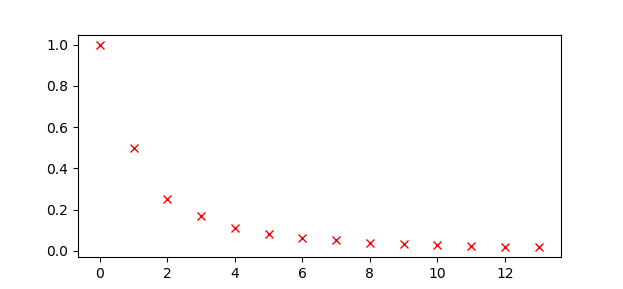
\includegraphics{minimalny_rozptyl.png}
\end{figure}

Vidíme, že pre rozmer $2k \times 2k$, uvedený v tabuľke a na grafe, je hodnota rozptylu $1/k^2$. Ukážeme, že to platí vo všeobecnosti.

\begin{prop}
Pre optimálnu maticu návrhu rozmeru $2k \times 2k$ je hodnota Gaussovho-Markovho odhadu rozdielu medzi efektami $1/k^2$.
\end{prop}

\begin{dokaz}
Nech $B$ je optimálna matica návrhu rozmeru $2k \times 2k$ spĺňajúca hypotézu (\ref{hypoteza1}). Označme $X$ maticu lineárnej regresie pre návrh $B$. Hodnotu rozptylu $m$ vypočítame ako $h^T M^- h$,
kde $M = X^T X$ je informačná matica lineárnej regresie a vektor $h = (0, 0, \ldots, -1, 1)^T $ zodpovedá rozdielu dvoch efektov. Ako vyzerajú posledné dva stĺpce matice $M$?

Matica $X$ je rozmeru $(4k + 2) \times (4k + 2)$, pričom prvých $2k$ riadkov zodpovedá $2k$ riadkom návrhu $B$, druhých $2k$ riadkov zodpovedá $2k$ stĺpcom návrhu $B$,
a posledné dva riadky zodpovedajú efektu na jednotlivých pozíciách návrhu $B$. Posledné dva stĺpce súčinu $X^T X$ zodpovedajú násobkom riadkov $X^T$ (stĺpcov $X$) s dvoma stĺpcami $X$ zodpovedajúcimi efektu.
Ak riadok, ktorým násobíme, je jeden zo $4k$ riadkov zodpovedajúcich stĺpcu alebo riadku návrhu $B$, hodnota súčinu bude predstavovať počet toho ktorého efektu v danom stĺpci alebo riadku.
Tá je podľa hypotézy (\ref{hypoteza1}) práve $k$ pre oba efekty. Ak navzájom násobíme riadok a stĺpec zodpovedajúci efektu, hodnota bude $0$, ak ide o rozdielne efekty,
alebo celkový počet daného efektu v návrhu $B$, ak ide o ten istý efekt. Počet efektu v optimálnom návrhu je podľa hypotézy $2k^2$.
Matica $X^T X$ je symetrická, preto jej posledné dva riadky budú rovnaké ako posledné dva stĺpce.

Posledné dva riadky matice $M = X^T X$ pre maticu návrhu $B$ rozmeru $2k \times 2k$ majú teda tvar:

\begin{center}
$
\begin{bmatrix}
k & k & \ldots & k & 2k^2 & 0 & \\
k & k & \ldots & k & 0 & 2k^2 & \\
\end{bmatrix}
$.
\end{center}

Napr. takto vyzerá matica $M$ pre optimálne návrhy rozmerov $2$ a $4$:

\begin{center}
$
\begin{bmatrix}
2 & 0 & 1 & 1 & 1 & 1 \\
0 & 2 & 1 & 1 & 1 & 1 \\
1 & 1 & 2 & 0 & 1 & 1 \\
1 & 1 & 0 & 2 & 1 & 1 \\
1 & 1 & 1 & 1 & 2 & 0 \\
1 & 1 & 1 & 1 & 0 & 2 \\
\end{bmatrix}
$,
$
\begin{bmatrix}
4 & 0 & 0 & 0 & 1 & 1 & 1 & 1 & 2 & 2 \\
0 & 4 & 0 & 0 & 1 & 1 & 1 & 1 & 2 & 2 \\
0 & 0 & 4 & 0 & 1 & 1 & 1 & 1 & 2 & 2 \\
0 & 0 & 0 & 4 & 1 & 1 & 1 & 1 & 2 & 2 \\
1 & 1 & 1 & 1 & 4 & 0 & 0 & 0 & 2 & 2 \\
1 & 1 & 1 & 1 & 0 & 4 & 0 & 0 & 2 & 2 \\
1 & 1 & 1 & 1 & 0 & 0 & 4 & 0 & 2 & 2 \\
1 & 1 & 1 & 1 & 0 & 0 & 0 & 4 & 2 & 2 \\
2 & 2 & 2 & 2 & 2 & 2 & 2 & 2 & 8 & 0 \\
2 & 2 & 2 & 2 & 2 & 2 & 2 & 2 & 0 & 8 \\
\end{bmatrix}
$.
\end{center}

Teraz dosadením ukážeme, že $h^T M^- h = (h^- M {h^-}^T)^-$. Ak to má platiť, musí platiť nasledovná rovnosť:

\begin{center}
$
h^- M {h^-}^T = h^- M {h^-}^T (h^- M {h^-}^T)^- h^- M {h^-}^T = h^- M {h^-}^T h^T M^- h h^- M {h^-}^T
$.
\end{center}

Pre vektor $v$ vo všeobecnosti platí, že $v^- = \frac{v^T}{v^T v}$. Pre náš vektor $h$ to znamená, že $h^- = h^T/2 = (0, 0, \ldots, -1/2, 1/2)$.
Ukážeme, že ${h^-}^T h^T$ a $h h^-$ vo vzorci vyššie dávajú tú istú maticu.

\begin{center}
$
{h^-}^T h^T = 
\begin{bmatrix}
0 \\
0 \\
\vdots \\
-1/2 \\
1/2 \\
\end{bmatrix}
\begin{bmatrix}
0 & 0 & \ldots & -1 & 1 \\
\end{bmatrix}
=
\begin{bmatrix}
0 & 0 & \ldots & 0 & 0 \\
0 & 0 & \ldots & 0 & 0 \\
\vdots && \ddots \\
0 & 0 & \ldots & 1/2 & -1/2 \\
0 & 0 & \ldots & -1/2 & 1/2 \\
\end{bmatrix}
$,
\end{center}

\begin{center}
$
h h^- = 
\begin{bmatrix}
0 \\
0 \\
\vdots \\
-1 \\
1 \\
\end{bmatrix}
\begin{bmatrix}
0 & 0 & \ldots & -1/2 & 1/2 \\
\end{bmatrix}
=
\begin{bmatrix}
0 & 0 & \ldots & 0 & 0 \\
0 & 0 & \ldots & 0 & 0 \\
\vdots && \ddots \\
0 & 0 & \ldots & 1/2 & -1/2 \\
0 & 0 & \ldots & -1/2 & 1/2 \\
\end{bmatrix}
$.
\end{center}

Označme túto maticu $H$. Teraz ukážeme, že $HM = MH$.

\begin{center}
$
HM = 
\begin{bmatrix}
0 & 0 & \ldots & 0 & 0 \\
0 & 0 & \ldots & 0 & 0 \\
\vdots && \ddots \\
0 & 0 & \ldots & 1/2 & -1/2 \\
0 & 0 & \ldots & -1/2 & 1/2 \\
\end{bmatrix}
\begin{bmatrix}
&&& k & k \\
&&& \vdots & \vdots \\
&&& k & k \\
k & \ldots & k & 2k^2 & 0 \\
k & \ldots & k & 0 & 2k^2 \\
\end{bmatrix}
=
\begin{bmatrix}
0 & 0 & \ldots & 0 & 0 \\
0 & 0 & \ldots & 0 & 0 \\
\vdots && \ddots \\
0 & 0 & \ldots & k^2 & -k^2 \\
0 & 0 & \ldots & -k^2 & k^2 \\
\end{bmatrix}
$,
\end{center}

\begin{center}
$
MH = 
\begin{bmatrix}
&&& k & k \\
&&& \vdots & \vdots \\
&&& k & k \\
k & \ldots & k & 2k^2 & 0 \\
k & \ldots & k & 0 & 2k^2 \\
\end{bmatrix}
\begin{bmatrix}
0 & 0 & \ldots & 0 & 0 \\
0 & 0 & \ldots & 0 & 0 \\
\vdots && \ddots \\
0 & 0 & \ldots & 1/2 & -1/2 \\
0 & 0 & \ldots & -1/2 & 1/2 \\
\end{bmatrix}
=
\begin{bmatrix}
0 & 0 & \ldots & 0 & 0 \\
0 & 0 & \ldots & 0 & 0 \\
\vdots && \ddots \\
0 & 0 & \ldots & k^2 & -k^2 \\
0 & 0 & \ldots & -k^2 & k^2 \\
\end{bmatrix}
$.
\end{center}

Takisto platí, že:

\begin{center}
$
h^- H =
\begin{bmatrix}
0 & 0 & \ldots & -1/2 & 1/2 \\
\end{bmatrix}
\begin{bmatrix}
0 & 0 & \ldots & 0 & 0 \\
0 & 0 & \ldots & 0 & 0 \\
\vdots && \ddots \\
0 & 0 & \ldots & 1/2 & -1/2 \\
0 & 0 & \ldots & -1/2 & 1/2 \\
\end{bmatrix}
=
\begin{bmatrix}
0 & 0 & \ldots & -1/2 & 1/2 \\
\end{bmatrix}
= h^-
$,
\end{center}

\begin{center}
$
H {h^-}^T =
\begin{bmatrix}
0 & 0 & \ldots & 0 & 0 \\
0 & 0 & \ldots & 0 & 0 \\
\vdots && \ddots \\
0 & 0 & \ldots & 1/2 & -1/2 \\
0 & 0 & \ldots & -1/2 & 1/2 \\
\end{bmatrix}
\begin{bmatrix}
0 \\
0 \\
\vdots \\
-1/2 \\
1/2 \\
\end{bmatrix}
=
\begin{bmatrix}
0 \\
0 \\
\vdots \\
-1/2 \\
1/2 \\
\end{bmatrix}
= {h^-}^T
$.
\end{center}

Dosaďme:

\begin{center}
$
h^- M {h^-}^T h^T M^- h h^- M {h^-}^T = h^- M H M^- H M {h^-}^T = h^- H M M^- M H {h^-}^T = h^- H M H {h^-}^T = h^- M {h^-}^T
$.
\end{center}

Takže naozaj platí $h^T M^- h = (h^- M {h^-}^T)^-$, resp. $(h^T M^- h)^- = h^- M {h^-}^T$ . Hodnotu $h^- M {h^-}^T$ vieme vypočítať:

\begin{center}
$
h^- M {h^-}^T = 
\begin{bmatrix}
0 & 0 & \ldots & -1/2 & 1/2 \\
\end{bmatrix}
\begin{bmatrix}
&&& k & k \\
&&& \vdots & \vdots \\
&&& k & k \\
k & \ldots & k & 2k^2 & 0 \\
k & \ldots & k & 0 & 2k^2 \\
\end{bmatrix}
\begin{bmatrix}
0 \\
0 \\
\vdots \\
-1/2 \\
1/2 \\
\end{bmatrix}
=
\begin{bmatrix}
0 & 0 & \ldots & -k^2 & k^2 \\
\end{bmatrix}
\begin{bmatrix}
0 \\
0 \\
\vdots \\
-1/2 \\
1/2 \\
\end{bmatrix}
= k^2/2 + k^2/2 = k^2
$.
\end{center}

Hodnota $x^-$ pre skalár $x$ je rovná $1/x$, preto $h^T M^- h = (h^- M {h^-}^T)^- = 1/k^2$. $\square$

\end{dokaz}

\begin{com}
Pri návrhoch nepárneho štvorcového rozmeru dôkaz zlyhá na rovnosti $HM = MH$.
Infomačná matica $M$ totiž pri nepárnom rozmere nemá natoľko vhodnú štruktúru ako pri párnom.
\end{com}

\subsection{Reprezentácia bipartitným grafom}

Ako sme avizovali na začiatku kapitoly, návrh nami opisovaného experimentu možno reprezentovať aj bipartitným grafom.
Tak ako v maticovej reprezentácii zodpovedali riadky dobrovoľníkom a stĺpce liečivám, podobne v bipartitnom grafe budú dobrovoľníci 
zodpovedať jednej partícii a liečivá druhej. Hrana sa medzi dvoma bodmi nachádza práve vtedy, keď pozícii tejto dvojice v matici návrhu zodpovedá nami zvolený spôsob ošetrenia.
Grafy zodpovedajúce jednému či druhému ošetreniu sú navzájom disjunktné a ich zjednotením získame kompletný bipartitný graf, t. j tieto dva grafy sú si navzájom doplnkami.
V zvyšku podkapitoly budeme tieto grafy označovať $\mathcal{G}$ a $\mathcal{G}'$.

Napríklad nasledovnej matici návrhu experimentu

\begin{center}
$
\begin{bmatrix}
1 & 0 & 0 \\
0 & 1 & 0 \\
\end{bmatrix}
$
\end{center}

priradíme dva grafy, jeden zodpovedajúci ošetreniu $1$:

\begin{center}

\begin {tikzpicture}[-latex, auto, node distance = 2 cm and 5cm, on grid, thick,
  state/.style ={ circle ,top color = white , bottom color = white, draw, black, text=black , minimum width = 0.8 cm}
]
  \begin{scope}[start chain=going below,node distance=2cm]
    \foreach \i in {1, 2}
      \node[state,on chain] (l\i) {};
  \end{scope}
  \begin{scope}[xshift=4cm,yshift=1cm,start chain=going below,node distance=2cm]
    \foreach \i in {1, 2, 3}
      \node[state,on chain] (r\i) {};
  \end{scope}

  \draw[-, thick] (l1) -- (r1);
  \draw[-, thick] (l2) -- (r2);

\end{tikzpicture}

\end{center}

a druhý, komplementárny prvému, zodpovedajúci ošetreniu $0$:

\begin{center}

\begin {tikzpicture}[-latex, auto, node distance = 2 cm and 5cm, on grid, thick,
  state/.style ={ circle, top color = white ,bottom color = white, draw, black, text=black , minimum width = 0.8 cm}
]
  \begin{scope}[start chain=going below,node distance=2cm]
    \foreach \i in {1, 2}
      \node[state,on chain] (l\i) {};
  \end{scope}
  \begin{scope}[xshift=4cm,yshift=1cm,start chain=going below,node distance=2cm]
    \foreach \i in {1, 2, 3}
      \node[state,on chain] (r\i) {};
  \end{scope}

  \draw[-, thick] (l1) -- (r2);
  \draw[-, thick] (l1) -- (r3);
  \draw[-, thick] (l2) -- (r1);
  \draw[-, thick] (l2) -- (r3);

\end{tikzpicture}

\end{center}

Každú binárnu maticu návrhu $m \times n$, zodpovedajúcej experimentu, teda možno reprezentovať bipartitným grafom s partíciami veľkostí $m$ a $n$. 
Ekvivalentne, každý bipartitný graf reprezentuje binárnu maticu, a teda aj experiment opísaný v tejto práci.

Naše tvrdenia a hypotézy z predošlých podkapitol možno vďaka tejto reprezentácii prepísať do jazyka teórie grafov.

\begin{prop}
Nech $\mathcal{G}$ je bipartitný graf s partíciami veľkosti $m$ a $n$. 
Potom hodnota $h^T b$ v lineárnom modeli reprezentovanom týmto grafom je odhadnuteľná práve vtedy,
keď v oboch partíciách existuje aspoň jeden taký vrchol, ktorý ani v $\mathcal{G}$ ani v $\mathcal{G}'$ nie je izolovaným bodom.
\end{prop}

\begin{dokaz}
Nech $B$ je matica návrhu experimentu. Potom podľa tvrdenia (\ref{statement 1})
hodnota $h^T b$ je odhadnuteľná $\Leftrightarrow$ v $B$ existuje aspoň jeden riadok a aspoň jeden stĺpec taký,
ktorý má aspoň jednu $0$ a aspoň jednu $1$ $\Leftrightarrow$ tento riadok a stĺpec bude zodpovedať vrcholu,
ktorý má hrany aj v $\mathcal{G}$ aj v $\mathcal{G}'$ $\Leftrightarrow$ v oboch partíciách $\mathcal{G}$ existuje taký vrchol, ktorý má hranu aj v $\mathcal{G}$ aj v $\mathcal{G}'$. $\square$
\end{dokaz}

\begin{defin}
Bipartitný graf $\mathcal{G}$ nazývame optimálnym, ak matica návrhu experimentu $B$ opísaná týmto grafom je optimálna v zmysle definície (\ref{optimal matrix definition}).
\end{defin}

\begin{hypoteza}
Nech $\mathcal{G}$ je bipartitný graf s partíciami veľkosti $2k$ a $2k$.
Potom $\mathcal{G}$ je optimálny práve vtedy, keď $\mathcal{G}$ je $k$-regulárny.

Nech $\mathcal{G}$ je bipartitný graf s partíciami veľkosti $2k + 1$ a $2k + 1$.
Potom $\mathcal{G}$ je optimálny práve vtedy, keď $\mathcal{G}$ je $k$-regulárny alebo $(k + 1)$-regulárny.
\end{hypoteza}

\begin{dokaz}
Nech $B$ je matica návrhu experimentu rozmeru $2k \times 2k$. Potom podľa hypotézy (\ref{hypoteza1})
$B$ je optimálna $\Leftrightarrow$ v každom riadku a stĺpci $B$ sa nachádza práve $k$ núl a práve $k$ jednotiek $\Leftrightarrow$
z každého vrchola $\mathcal{G}$ zodpovedajúceho riadku $B$ bude vychádzať práve $k$ hrán,
z každého vrchola zodpovedajúceho stĺpcu $\mathcal{G}$ bude vychádzať práve $k$ hrán $\Leftrightarrow$ $\mathcal{G}$ je $k$-regulárny.

Ekvivalentne tvrdenie ukážeme pre rozmer $(2k + 1) \times (2k + 1)$. $\square$
\end{dokaz}

\begin{hypoteza}
Nech $\mathcal{G}$ je bipartitný graf.

Postačujúcou podmienkou optimality $\mathcal{G}$ s veľkosťami partícií $2k$ a $2l$ je, ak má $\mathcal{G}$ práve $2kl$ hrán,
pričom každý z $2k$ vrcholov prvej partície má stupeň $l$ a každý z $2l$ vrcholov druhej partície má stupeň $k$.

Postačujúcou podmienkou optimality $\mathcal{G}$ s veľkosťami partícií $2l + 1$ a $2k$ je, ak má $\mathcal{G}$ práve $(2l + 1)k$ hrán,
pričom každý z $(2l + 1)$ vrcholov prvej partície má stupeň $k$, $k$ vrcholov druhej partície má stupeň $l + 1$ a zvyšných $k$ vrcholov má stupeň $l$.

Ďalej nech bez ujmy na všeobecnosti $k < l$.

Postačujúcou podmienkou optimality $\mathcal{G}$ s veľkosťami partícií $2k + 1$ a $2l + 1$, ak $\mathcal{G}$ alebo $\mathcal{G}'$ má práve $(l + 1)(2k + 1)$ hrán,
pričom každý z $2k + 1$ vrcholov prvej partície má stupeň $l + 1$, $l + k + 1$ vrcholov druhej partície má stupeň $k + 1$ a zvyšných $l - k$ vrcholov má stupeň $k$.
\end{hypoteza}

\begin{dokaz}
Podobne ako pri dôkaze predošlého tvrdenia, jednotlivé grafy jednoznačne priradíme binárnym maticiam. Tvrdenie potom vyplynie z hypotézy (\ref{hypoteza2}). $\square$
\end{dokaz}

Reprezentácia bipartitným grafom nám pri našich súčasných poznatkoch o riadkovo-stĺpcovom aditívnom modeli s dvoma typmi ošetrení neponúkla ďalšie hlbšie závery, 
avšak ponúkla nám prísľub, že pri našom ďalšom skúmaní v budúcnosti sa budeme môcť oprieť aj o poznatky z teórie grafov.

  % \newpage
  % \section{Porovnanie výsledkov}

Hello world

	\newpage
  \section*{Záver}
    \addcontentsline{toc}{section}{Záver}
    \markboth{ZÁVER}{ZÁVER} 
    V práci sme skúmali tzv. riadkovo-stĺpcové návrhy štatistických experimentov. 
Vzali sme na seba rolu experimentátora a jedným z našich cieľov bolo nájsť ten návrh experimentu, ktorý nám ponúkne čo najvhodnejšie výsledky.

V praktickej časti sme najprv identifikovali tie návrhy, v ktorých je možné odhadnúť žiadanú veličinu - kontrast medzi dvoma možnými ošetreniami. 
Následne sme určili, v ktorých návrhoch vieme tento kontrast odhadnúť čo najpresnejšie, a vytvorili sme jednoduchý algoritmus, ako tieto návrhy zostrojiť pre ľubovoľný rozmer. 
Algoritmus napísaný v jazyku \emph{python} sa nachádza v prílohe \hyperref[appendix:d]{D}.

Hoci sme ponúkli niekoľko zaujímavých záverov, priestor na bádanie sme zďaleka nevyčerpali. 
Pripomíname, že sme sa obmedzili na veľmi konkrétnu triedu experimentov. Mechanizmy, ktoré sme pri výskume použili, však majú potenciál byť využité aj pri iných druhoch experimentov.

Mohli by sme napríklad pracovať nie s dvoma typmi ošetrení, ako tomu bolo v našej práci, ale s troma a viac. 
Ďalším z možných rozšírení by bolo “zakázanie” niektorých kombinácií dvoch faktorov a jeho vplyv na optimálny návrh experimentu.

Tiež sme naplno nevyužili potenciál teórie grafov, ktorá sa v tematike optimálneho návrhu experimentov využíva často. 
Grafové metódy boli použité napr. pri návrhoch blokových experimentov s mnohými ošetreniami (viď napr. \cite{cheng, bailey}) 
alebo tzv. aproximatívnych návrhoch pre modely so špeciálnou množinou kontrastov medzi viacerými ošetreniami (viď \cite{rosa}). 
Do budúcnosti by bolo možné preskúmať súvislosti grafovej reprezentácie binárnych riadkovo-stĺpcových návrhov s týmito grafovými prístupmi k navrhovaniu experimentov.

Jedná sa o problematiku, ktorej nebolo venované toľko článkov a publikácií, ako iným, populárnejším témam. 
Nech aj to je pre nás motiváciou k ďalšiemu bádaniu.
  
  \newpage
  \renewcommand{\refname}{Zoznam použitej literatúry}
  \begin{thebibliography}{99}

	\bibitem{pazman} Pázman, A., Lacko, V.: {\it Prednášky z regresných modelov}, Vydavateľstvo UK, Bratislava, 2012, 2015

	\bibitem{kniha} Freedman, David: {\it Statistical models: Theory and practice}, Cambridge University Press, New York, 2005

	\bibitem{kniha} Rencher, Alvin C.: {\it Methods of Multivariate Analysis}, John Wiley \& Sons, New York, 2002

	\bibitem{yan} Yan, Xin: {\it Linear Regression Analysis: Theory and Computing}, World Scientific Publishing Co. Pte. Ltd., Singapore, 2009

	\bibitem{kniha} \url{http://oeis.org/A002724}

	\bibitem{cheng} Cheng, C.S.: {\it Maximizing the total number of spanning trees in a graph: two related problems in graph theory and optimum design theory},
	Department of Statistics, University of California, Berkeley, California 94720, USA

	\bibitem{bailey} Bailey, R.A., Cameron, P.J.: {\it Combinatorics of optimal designs. Surveys in Combinatorics}, London Mathematical Society Lecture Note Series 365, 2009

	\bibitem{rosa} Rosa, S.: {\it Optimal designs for treatment comparisons represented by graphs}, dostupné na internete: \url{https://link.springer.com/article/10.1007%2Fs10182-017-0312-5}

\end{thebibliography}

  
	\newpage
  \appendix
  \section*{Príloha A} 
    \label{appendix:a}
    \addcontentsline{toc}{section}{Príloha A}
    \markboth{Príloha A}{Príloha A}
    \textbf{Návrhy rozmeru $3 \times 3$, pre ktoré nie je možné odhadnúť hodnotu $h^T b$}

\begin{center}
$
\begin{bmatrix}
0 & 0 & 0 \\ 
0 & 0 & 0 \\ 
0 & 0 & 0 \\ 
\end{bmatrix}
,
\begin{bmatrix}
0 & 0 & 0 \\
1 & 1 & 1 \\
0 & 0 & 0 \\
\end{bmatrix}
,
\begin{bmatrix}
1 & 1 & 1 \\
0 & 0 & 0 \\
0 & 0 & 0 \\
\end{bmatrix}
,
\begin{bmatrix}
1 & 1 & 1 \\
1 & 1 & 1 \\
0 & 0 & 0 \\
\end{bmatrix}
,
\begin{bmatrix}
0 & 0 & 0 \\
0 & 0 & 0 \\
0 & 0 & 0 \\
\end{bmatrix}
,
\begin{bmatrix}
0 & 0 & 0 \\
0 & 0 & 0 \\
1 & 1 & 1 \\
\end{bmatrix}
,
\begin{bmatrix}
0 & 0 & 0 \\
1 & 1 & 1 \\
0 & 0 & 0 \\
\end{bmatrix}
$
\end{center}
\begin{center}
$
\begin{bmatrix}
0 & 0 & 0 \\
1 & 1 & 1 \\
1 & 1 & 1 \\
\end{bmatrix}
,
\begin{bmatrix}
0 & 0 & 1 \\
0 & 0 & 1 \\
0 & 0 & 1 \\
\end{bmatrix}
,
\begin{bmatrix}
0 & 1 & 0 \\
0 & 1 & 0 \\
0 & 1 & 0 \\
\end{bmatrix}
,
\begin{bmatrix}
0 & 1 & 1 \\
0 & 1 & 1 \\
0 & 1 & 1 \\
\end{bmatrix}
,
\begin{bmatrix}
1 & 0 & 0 \\
1 & 0 & 0 \\
1 & 0 & 0 \\
\end{bmatrix}
,
\begin{bmatrix}
1 & 0 & 1 \\
1 & 0 & 1 \\
1 & 0 & 1 \\
\end{bmatrix}
,
\begin{bmatrix}
1 & 1 & 0 \\
1 & 1 & 0 \\
1 & 1 & 0 \\
\end{bmatrix}
$
\end{center}
\begin{center}
$
\begin{bmatrix}
1 & 1 & 1 \\
0 & 0 & 0 \\
0 & 0 & 0 \\
\end{bmatrix}
,
\begin{bmatrix}
1 & 1 & 1 \\
0 & 0 & 0 \\
1 & 1 & 1 \\
\end{bmatrix}
,
\begin{bmatrix}
1 & 1 & 1 \\
1 & 1 & 1 \\
0 & 0 & 0 \\
\end{bmatrix}
,
\begin{bmatrix}
1 & 1 & 1 \\
1 & 1 & 1 \\
1 & 1 & 1 \\
\end{bmatrix}
$
\end{center}

  \newpage
  \section*{Príloha B}
    \label{appendix:b}
    \addcontentsline{toc}{section}{Príloha B}
    \markboth{Príloha B}{Príloha B}
    \renewcommand{\thesection}{A.\arabic{section}}
\renewcommand{\theequation}{A.\arabic{equation}}
\renewcommand{\thefigure}{A.\arabic{figure}}
\setcounter{equation}{0}

\textbf{Niektoré optimálne návrhy}

\begin{center}
$
\begin{bmatrix}
0 & 0 & 0 & 0 & 1 & 1 & 1 \\
0 & 0 & 0 & 1 & 0 & 1 & 1 \\
1 & 1 & 1 & 0 & 0 & 0 & 0 \\
\end{bmatrix}
,
\begin{bmatrix}
0 & 0 & 1 & 1 \\
0 & 0 & 1 & 1 \\
1 & 1 & 0 & 0 \\
1 & 1 & 0 & 0 \\
\end{bmatrix}
,
\begin{bmatrix}
0 & 0 & 0 & 1 & 1 \\ 
0 & 0 & 0 & 1 & 1 \\ 
1 & 1 & 1 & 0 & 0 \\ 
1 & 1 & 1 & 0 & 0 \\ 
\end{bmatrix}
,
\begin{bmatrix}
0 & 0 & 0 & 1 & 1 \\
0 & 0 & 0 & 1 & 1 \\
0 & 1 & 1 & 0 & 0 \\
1 & 0 & 1 & 0 & 0 \\
1 & 1 & 0 & 0 & 0 \\
\end{bmatrix}
$
\end{center}
\begin{center}
$
\begin{bmatrix}
0 & 0 & 1 & 1 \\ 
0 & 0 & 1 & 1 \\ 
0 & 0 & 1 & 1 \\ 
1 & 1 & 0 & 0 \\ 
1 & 1 & 0 & 0 \\ 
1 & 1 & 0 & 0 \\ 
\end{bmatrix}
,
\begin{bmatrix}
0 & 0 & 0 & 1 & 1 \\ 
0 & 0 & 0 & 1 & 1 \\ 
0 & 0 & 0 & 1 & 1 \\ 
1 & 1 & 1 & 0 & 0 \\ 
1 & 1 & 1 & 0 & 0 \\ 
1 & 1 & 1 & 0 & 0 \\ 
\end{bmatrix}
,
\begin{bmatrix}
0 & 0 & 0 & 1 & 1 & 1 \\ 
0 & 0 & 0 & 1 & 1 & 1 \\ 
0 & 0 & 0 & 1 & 1 & 1 \\ 
1 & 1 & 1 & 0 & 0 & 0 \\ 
1 & 1 & 1 & 0 & 0 & 0 \\ 
1 & 1 & 1 & 0 & 0 & 0 \\ 
\end{bmatrix}
,
\begin{bmatrix}
1 & 1 & 1 & 1 & 0 & 0 & 0 & 0 \\
1 & 1 & 1 & 1 & 0 & 0 & 0 & 0 \\
1 & 1 & 1 & 1 & 0 & 0 & 0 & 0 \\
1 & 1 & 1 & 1 & 0 & 0 & 0 & 0 \\
0 & 0 & 0 & 0 & 1 & 1 & 1 & 1 \\
0 & 0 & 0 & 0 & 1 & 1 & 1 & 1 \\
0 & 0 & 0 & 0 & 1 & 1 & 1 & 1 \\
0 & 0 & 0 & 0 & 1 & 1 & 1 & 1 \\
\end{bmatrix}
$
\end{center}

\begin{center}
$
\begin{bmatrix}
1 & 1 & 1 & 1 & 1 & 1 & 1 & 0 & 0 & 0 & 0 & 0 & 0 & 0 \\
1 & 1 & 1 & 1 & 1 & 1 & 1 & 0 & 0 & 0 & 0 & 0 & 0 & 0 \\
1 & 1 & 1 & 1 & 1 & 1 & 1 & 0 & 0 & 0 & 0 & 0 & 0 & 0 \\
1 & 1 & 1 & 1 & 1 & 1 & 1 & 0 & 0 & 0 & 0 & 0 & 0 & 0 \\
1 & 1 & 1 & 1 & 1 & 1 & 1 & 0 & 0 & 0 & 0 & 0 & 0 & 0 \\
1 & 1 & 1 & 1 & 1 & 1 & 1 & 0 & 0 & 0 & 0 & 0 & 0 & 0 \\
1 & 1 & 1 & 1 & 1 & 1 & 1 & 0 & 0 & 0 & 0 & 0 & 0 & 0 \\
0 & 0 & 0 & 0 & 0 & 0 & 0 & 1 & 1 & 1 & 1 & 1 & 1 & 1 \\
0 & 0 & 0 & 0 & 0 & 0 & 0 & 1 & 1 & 1 & 1 & 1 & 1 & 1 \\
0 & 0 & 0 & 0 & 0 & 0 & 0 & 1 & 1 & 1 & 1 & 1 & 1 & 1 \\
0 & 0 & 0 & 0 & 0 & 0 & 0 & 1 & 1 & 1 & 1 & 1 & 1 & 1 \\
0 & 0 & 0 & 0 & 0 & 0 & 0 & 1 & 1 & 1 & 1 & 1 & 1 & 1 \\
0 & 0 & 0 & 0 & 0 & 0 & 0 & 1 & 1 & 1 & 1 & 1 & 1 & 1 \\
0 & 0 & 0 & 0 & 0 & 0 & 0 & 1 & 1 & 1 & 1 & 1 & 1 & 1 \\
\end{bmatrix}
$
\end{center}

\begin{center}
$
\begin{bmatrix}
1 & 1 & 1 & 1 & 1 & 1 & 1 & 1 & 0 & 0 & 0 & 0 & 0 & 0 & 0 & 0 & 0 \\
1 & 1 & 1 & 1 & 1 & 1 & 1 & 1 & 0 & 0 & 0 & 0 & 0 & 0 & 0 & 0 & 0 \\
1 & 1 & 1 & 1 & 1 & 1 & 1 & 1 & 0 & 0 & 0 & 0 & 0 & 0 & 0 & 0 & 0 \\
1 & 1 & 1 & 1 & 1 & 1 & 1 & 1 & 0 & 0 & 0 & 0 & 0 & 0 & 0 & 0 & 0 \\
1 & 1 & 1 & 1 & 1 & 1 & 1 & 1 & 0 & 0 & 0 & 0 & 0 & 0 & 0 & 0 & 0 \\
1 & 1 & 1 & 1 & 1 & 1 & 1 & 1 & 0 & 0 & 0 & 0 & 0 & 0 & 0 & 0 & 0 \\
1 & 1 & 1 & 1 & 1 & 1 & 1 & 1 & 0 & 0 & 0 & 0 & 0 & 0 & 0 & 0 & 0 \\
1 & 1 & 1 & 1 & 1 & 1 & 1 & 1 & 0 & 0 & 0 & 0 & 0 & 0 & 0 & 0 & 0 \\
0 & 0 & 0 & 0 & 0 & 0 & 0 & 0 & 0 & 1 & 1 & 1 & 1 & 1 & 1 & 1 & 1 \\
0 & 0 & 0 & 0 & 0 & 0 & 0 & 0 & 1 & 0 & 1 & 1 & 1 & 1 & 1 & 1 & 1 \\
0 & 0 & 0 & 0 & 0 & 0 & 0 & 0 & 1 & 1 & 0 & 1 & 1 & 1 & 1 & 1 & 1 \\
0 & 0 & 0 & 0 & 0 & 0 & 0 & 0 & 1 & 1 & 1 & 0 & 1 & 1 & 1 & 1 & 1 \\
0 & 0 & 0 & 0 & 0 & 0 & 0 & 0 & 1 & 1 & 1 & 1 & 0 & 1 & 1 & 1 & 1 \\
0 & 0 & 0 & 0 & 0 & 0 & 0 & 0 & 1 & 1 & 1 & 1 & 1 & 0 & 1 & 1 & 1 \\
0 & 0 & 0 & 0 & 0 & 0 & 0 & 0 & 1 & 1 & 1 & 1 & 1 & 1 & 0 & 1 & 1 \\
0 & 0 & 0 & 0 & 0 & 0 & 0 & 0 & 1 & 1 & 1 & 1 & 1 & 1 & 1 & 0 & 1 \\
0 & 0 & 0 & 0 & 0 & 0 & 0 & 0 & 1 & 1 & 1 & 1 & 1 & 1 & 1 & 1 & 0 \\
\end{bmatrix}
$
\end{center}

  \newpage
  \section*{Príloha C}
    \label{appendix:c}
    \addcontentsline{toc}{section}{Príloha C}
    \markboth{Príloha C}{Príloha C}
    \textbf{Vytvorenie optimálnej štvorcovej matice pre rozmer $n \times n$}

\begin{lstlisting}[language=Python, basicstyle=\footnotesize]
def create_optimal_matrix(n):
    matrix = []
    if n % 2 == 0:
        for i in range(n):
            row = [0 for j in range(n)]
            for j in range(n//2):
                if i < n/2:
                    row[j] = 1
                else:
                    row[n - j - 1] = 1
            matrix.append(row)
    else:
        for i in range(n):
            row = [0 for j in range(n)]
            if i < n//2:
                for j in range(n//2):
                    row[j] = 1
            else:
                for j in range(n//2 + 1):
                    row[n - j - 1] = 1
                    row[i] = 0
                matrix.append(row)
    return matrix
\end{lstlisting}
    %\begin{comment}

  \newpage
  \section*{Príloha D}
    \label{appendix:d}
    \addcontentsline{toc}{section}{Príloha D}
    \markboth{Príloha D}{Príloha D}
    \textbf{Vytvorenie optimálnej štvorcovej matice pre rozmer $n \times n$}

\begin{lstlisting}[language=Python, basicstyle=\footnotesize]
def create_optimal_matrix(n):
    matrix = []
    if n % 2 == 0:
        for i in range(n):
            row = [0 for j in range(n)]
            for j in range(n//2):
                if i < n/2:
                    row[j] = 1
                else:
                    row[n - j - 1] = 1
            matrix.append(row)
    else:
        for i in range(n):
            row = [0 for j in range(n)]
            if i < n//2:
                for j in range(n//2):
                    row[j] = 1
            else:
                for j in range(n//2 + 1):
                    row[n - j - 1] = 1
                    row[i] = 0
                matrix.append(row)
    return matrix
\end{lstlisting}
%\end{comment}
\end{document}
